%% Springer Nature LaTeX template — npj Microgravity style.
%% sn-jnl.cls + sn-nature.bst ship with Springer Nature's template (see README.md).
\documentclass[pdflatex,sn-nature]{sn-jnl}

\usepackage{graphicx}
\usepackage{multirow}
\usepackage{amsmath,amssymb,amsfonts}
\usepackage{booktabs}
\usepackage{longtable}
\usepackage{textcomp}
\usepackage{url}

\graphicspath{{figures/}}

\begin{document}

\title[Spaceflight alters the tomato microbiome light-dependently]{Spaceflight
alters the tomato phyllosphere and rhizosphere microbiome in a light-dependent
manner: a multi-omics integration of ISS VEG-05}

%% TODO: confirm author list, ORCID(s), and affiliation before submission.
\author[1]{\fnm{Richard} \sur{Barker}}
\affil[1]{\orgname{[Affiliation --- TODO]}, \email{admin@cosecloud.com}}

\abstract{Spaceflight imposes unique stressors on plant-microbe interactions, but
the coordinated responses of host transcriptomes and associated microbiomes remain
poorly characterized. We analyzed tomato (\textit{Solanum lycopersicum} cv.\ Red
Robin) grown aboard the International Space Station (ISS) as part of the VEG-05
experiment, integrating 16S rRNA and ITS amplicon sequencing (OSD-766) with host
transcriptomics (OSD-767) across two tissues (leaf, adventitious root) and two
light treatments (red vs.\ blue). DADA2 processing yielded 348 bacterial and 77
fungal ASVs from 142 and 141 samples respectively. Spaceflight significantly
reshaped leaf bacterial communities (PERMANOVA \(R^2 = 0.42\), \(p = 0.001\)) and
increased bacterial alpha diversity (Observed ASVs: Flight 17.8--25.8 vs.\ Ground
10.0--15.2). The spaceflight transcriptional response was strongly light-dependent:
under blue light, 4{,}716 differentially expressed genes (DEGs) were detected in
leaves versus only 523 under red light. WGCNA identified a 169-gene adventitious
root module correlated with fungal dysbiosis (\(r = -0.85\), \(p_{\mathrm{adj}} =
0.001\)) but not with flight status (\(r = -0.38\), \(p = 0.32\)), representing a
microbe-driven host transcriptional signature independent of the direct spaceflight
stimulus. MOFA+ integration across three omics layers confirmed a dominant
flight-associated factor (48\% transcriptome variance) and revealed that the leaf
bacterial community was more responsive to spaceflight than the fungal community.
FAPROTAX functional prediction identified nitrogen fixation, methanotrophy, and
methanol oxidation as enriched functions in the bacterial community. These findings
demonstrate that spaceflight restructures plant-associated microbiomes in a tissue-
and light-specific manner, with implications for crop production systems in
long-duration space missions.}

\keywords{spaceflight, plant microbiome, multi-omics, VEG-05, tomato, WGCNA,
MOFA+, dysbiosis}

\maketitle

\section{Introduction}\label{sec:intro}

Plant-associated microbiomes play critical roles in nutrient acquisition, pathogen
protection, and stress tolerance \cite{bulgarelli2013}. In the context of
spaceflight, these interactions take on added significance: crops grown in
bioregenerative life support systems must maintain productive plant-microbe
partnerships under conditions of microgravity, altered fluid dynamics, elevated
radiation, and controlled-environment lighting \cite{wheeler2008}. The VEG-05
experiment aboard the International Space Station (ISS) provided a unique
opportunity to study these interactions in tomato (\textit{Solanum lycopersicum}),
a candidate crop for long-duration missions \cite{massa2024}.

Spaceflight has been shown to alter microbial community composition, gene
expression, and virulence in pure culture systems \cite{rosenzweig2015,voorhies2019a}.
However, the coordinated response of host plants and their associated microbiomes to
the spaceflight environment remains largely unexplored. Multi-omics integration
approaches such as MOFA+ (Multi-Omics Factor Analysis) \cite{argelaguet2020} and
WGCNA (Weighted Gene Co-expression Network Analysis) \cite{langfelder2008} offer
powerful frameworks for identifying coordinated variation across biological layers,
but have not been applied to spaceflight plant-microbiome studies.

Here we present an integrated analysis of the VEG-05 tomato microbiome (16S rRNA and
ITS amplicon sequencing, OSD-766) and host transcriptome (RNA-seq, OSD-767)
(Fig.~\ref{fig:1}). We characterize community health through diversity metrics and a
dysbiosis index, identify co-expression modules associated with microbial changes,
and infer the directionality of host-microbe interactions using a framework that
distinguishes host-driven, microbe-driven, and co-regulated responses.

\begin{figure}[htbp]
\centering
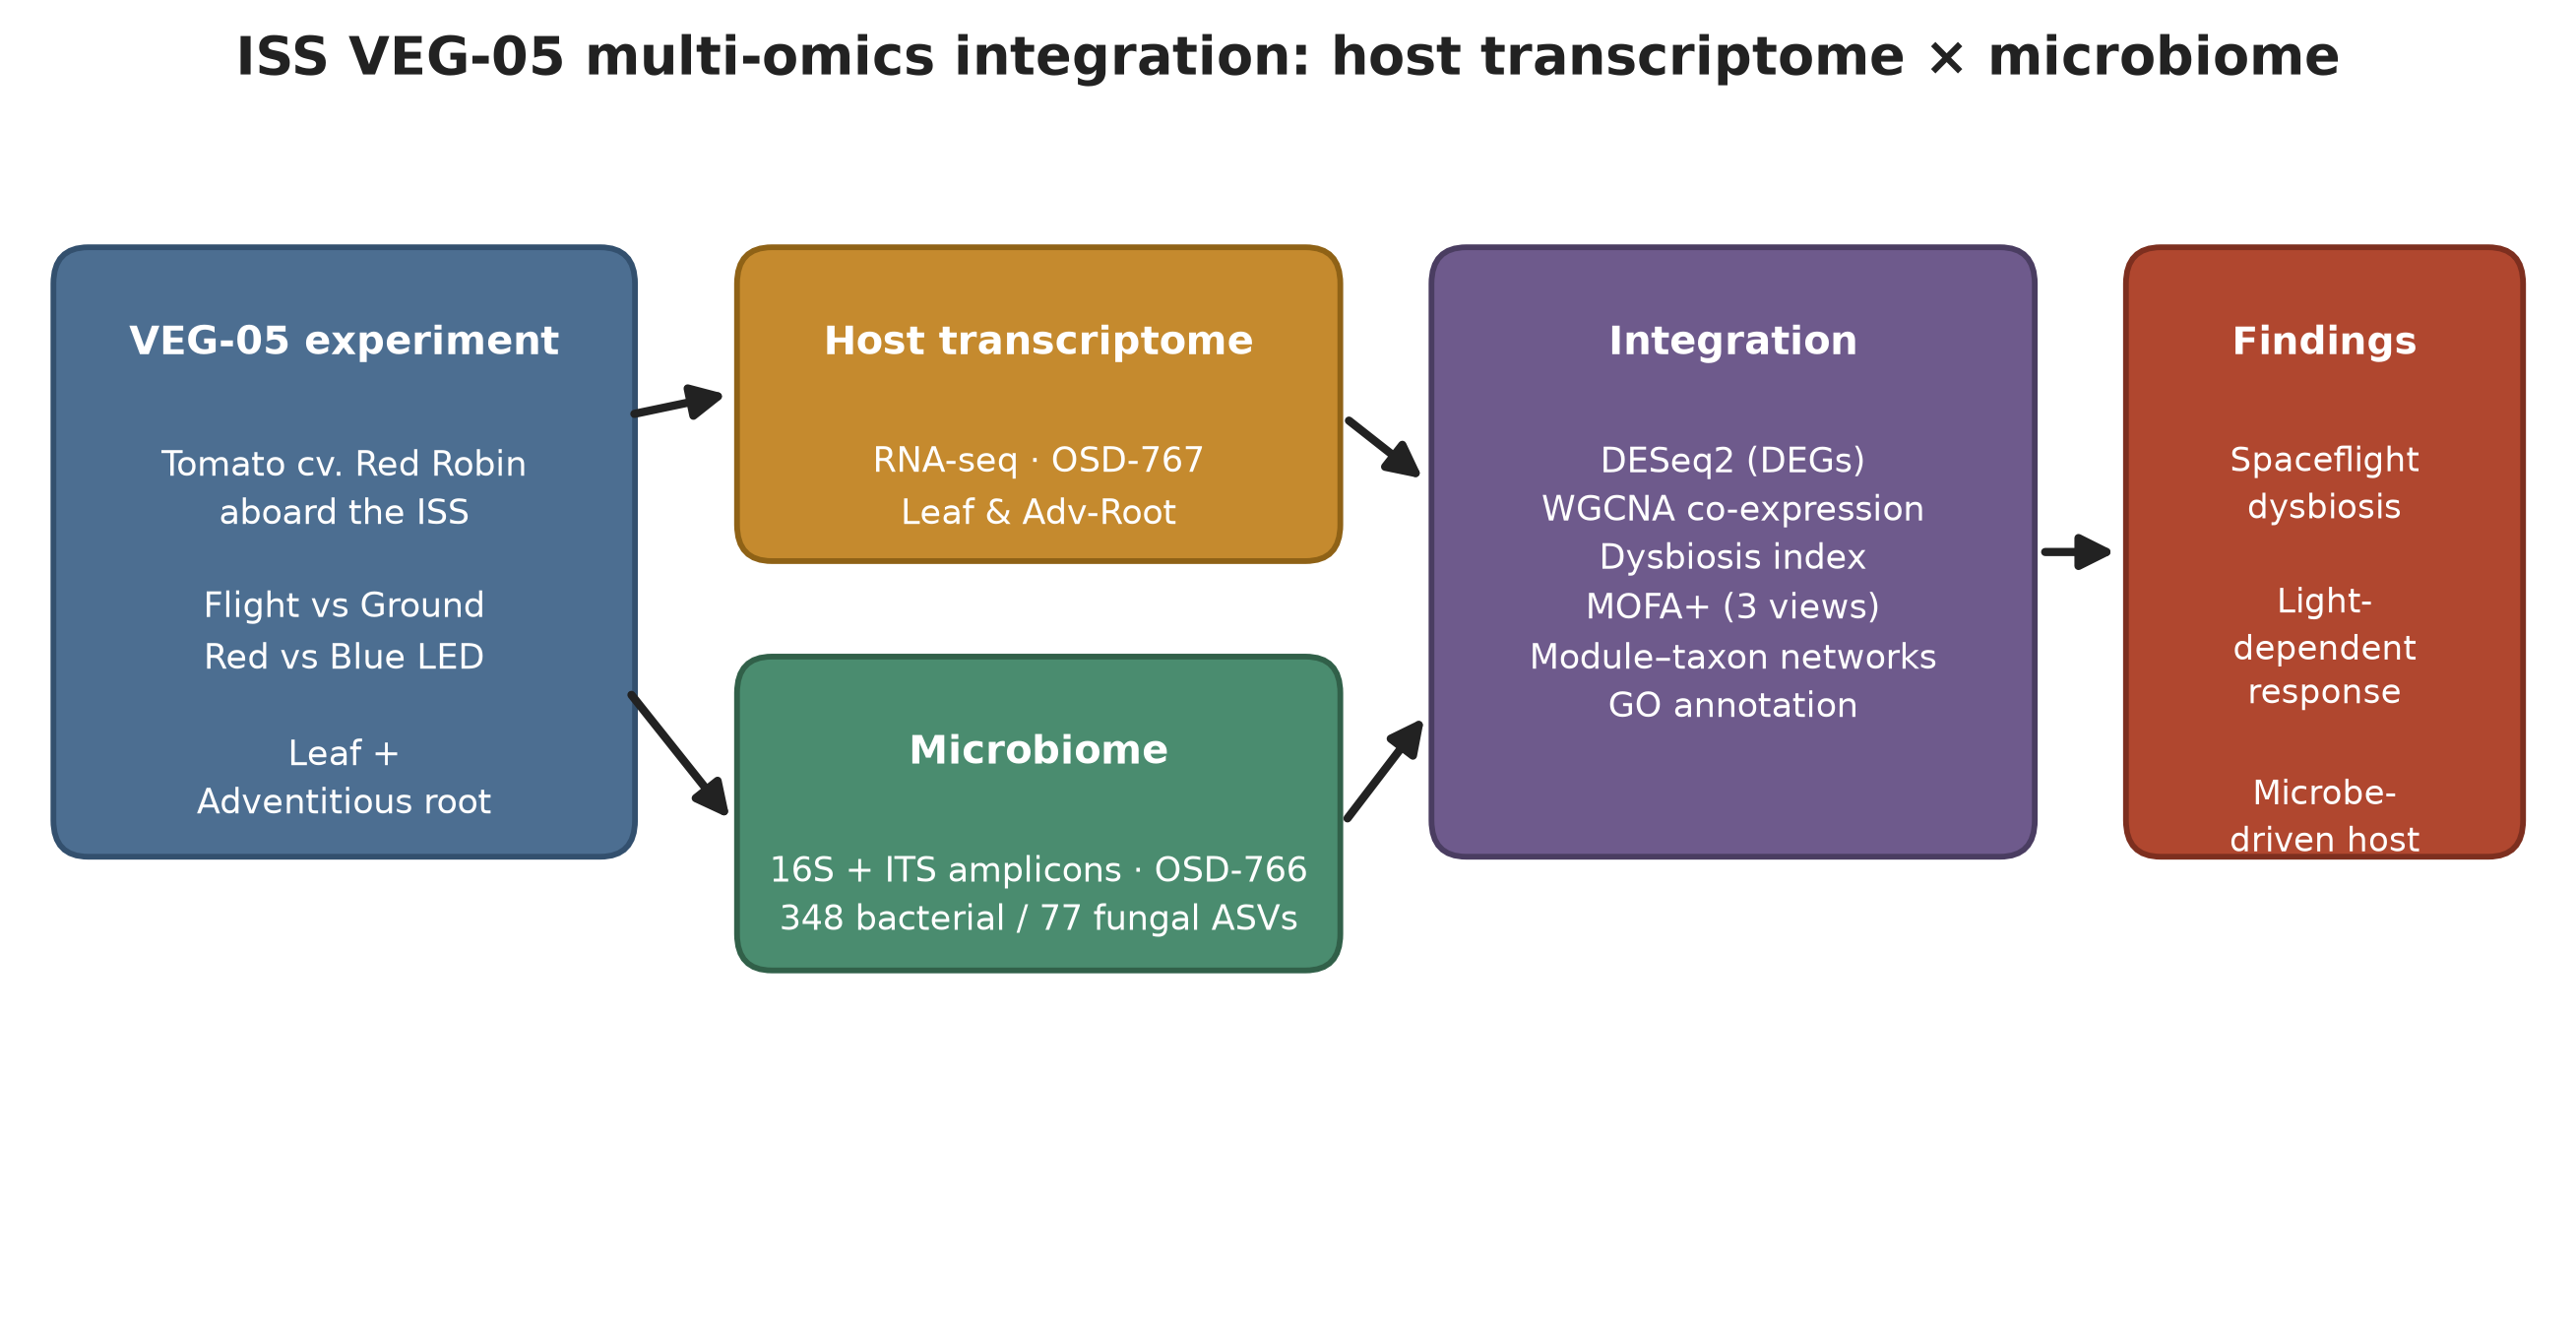
\includegraphics[width=\textwidth]{fig1_study_design.png}
\caption{\textbf{Study design and analysis overview.} The ISS VEG-05 experiment
(tomato cv.\ Red Robin; Flight vs Ground; red vs blue LED; leaf and adventitious
root) feeds two data streams --- host transcriptome (OSD-767) and microbiome
(OSD-766) --- combined through DESeq2, WGCNA, a dysbiosis index, MOFA+, and
module--taxon networks.}
\label{fig:1}
\end{figure}

\section{Methods}\label{sec:methods}

\subsection{Data acquisition and metadata}
Raw sequencing data and metadata were obtained from NASA's Open Science Data
Repository (OSDR): OSD-766 (microbiome amplicon sequencing) and OSD-767 (host
RNA-seq). The VEG-05 experiment grew tomato cv.\ Red Robin aboard the ISS under red
or blue LED lighting, with ground controls at Kennedy Space Center. Metadata were
parsed from ISA-Tab format, and a crosswalk table linking microbiome and RNA-seq
samples by plant ID, flight status, light treatment, and tissue was constructed.

\subsection{Microbiome amplicon processing}
16S rRNA (V4 region, 515F/806R primers) and ITS2 (ITS3F/ITS4 primers) reads were
processed using DADA2 v1.34.0 \cite{callahan2016} in R. For 16S, primers were
already removed; reads were truncated at 240 bp (R1) and 160 bp (R2) with maxEE = 2,
length-filtered to 200--260 bp, and pooled for denoising. Taxonomy was assigned
against SILVA 138.2 \cite{quast2013}. Chloroplast and mitochondrial ASVs were
removed prior to community analysis. For ITS, primers were removed with cutadapt
\cite{martin2011}; R2 reads were truncated at 180 bp due to quality degradation;
taxonomy was assigned against UNITE v7 (October 2017) \cite{koljalg2005}.

\subsection{Differential expression analysis}
RNA-seq count matrices were analyzed with DESeq2 \cite{love2014} separately for leaf
(21 samples) and adventitious root (15 samples; Table~S1). The design model included
flight status, light treatment, and their interaction. Log-fold changes were shrunk
with apeglm \cite{zhu2019} for main effects and ashr \cite{stephens2017} for subset
contrasts. DEGs were defined as \(p_{\mathrm{adj}} < 0.05\) and \(|\text{log2FC}|
\geq 1\).

\subsection{Community health metrics}
Alpha diversity (Observed ASVs, Shannon index) was computed on unfiltered data using
phyloseq \cite{mcmurdie2013}. Beta diversity was assessed via Bray-Curtis
dissimilarity and PERMANOVA (999 permutations) using vegan \cite{oksanen2024}. A
dysbiosis index was calculated as the Bray-Curtis distance of each flight sample to
the centroid of its corresponding ground control group, normalized by the mean
ground-ground distance. Differential abundance testing used ALDEx2
\cite{fernandes2013} with 128 Monte Carlo instances, requiring both Welch \(p <
0.05\) and \(|\text{effect size}| > 1\).

\subsection{WGCNA co-expression networks}
WGCNA \cite{langfelder2008} was applied to variance-stabilized transcriptome data
for each tissue separately. Soft-thresholding powers were selected to maximize
scale-free fit (Leaf: power = 20, \(R^2 = 0.72\); Adv-Root: power = 18, \(R^2 =
0.69\)). Module eigengenes were correlated with flight status, light treatment, and
16S/ITS dysbiosis indices. Hub genes were identified by module membership
(\(k_{\mathrm{ME}} > 0.8\)).

\subsection{MOFA+ multi-omics integration}
MOFA2 \cite{argelaguet2020} was trained on 21 leaf samples with matched data across
three views: transcriptome (2{,}000 most variable genes), 16S (348 ASVs), and ITS
(77 ASVs). The model was trained with 5 factors and default priors. Factor-trait
correlations were computed using Spearman's rank correlation with BH correction.

\subsection{Correlation networks and directionality inference}
Bipartite module-taxon networks were constructed by Spearman correlation between
WGCNA module eigengenes and ASV relative abundances (prevalence filter \(>20\%\), BH
correction). GO enrichment of WGCNA modules was performed using clusterProfiler's
enricher function \cite{yu2012} with tomato GO annotations from Ensembl Plants
(18{,}479 annotated genes). Directionality was classified as: host-driven
(correlated with flight/light but not dysbiosis), microbe-driven (correlated with
dysbiosis but not flight/light), or co-regulated (correlated with both).

\subsection{Functional prediction}
Bacterial functional profiles were predicted using FAPROTAX v1.2 \cite{louca2016}
with a custom Python implementation of the collapse algorithm. Fungal ecological
guilds were assigned using genus-level lookup tables based on FUNGuild
\cite{nguyen2016} categories.

\section{Results}\label{sec:results}

\subsection{Spaceflight reshapes leaf bacterial communities}
DADA2 processing of 16S rRNA reads yielded 544 ASVs from 142 samples (3{,}558{,}814
non-chimeric reads, 89.8\% retention). After removing chloroplast (38.9\% of reads)
and mitochondrial (21.5\%) sequences, 348 bacterial ASVs remained. ITS processing
yielded 77 fungal ASVs from 141 samples (160{,}316 reads, 15.8\% retention).

Spaceflight significantly altered leaf bacterial community composition (PERMANOVA:
\(R^2 = 0.42\), \(F = 4.02\), \(p = 0.001\), \(n = 21\)) and adventitious root
communities (\(R^2 = 0.33\), \(F = 2.93\), \(p = 0.001\), \(n = 15\); Table~S4). In
leaves, bacterial alpha diversity was higher in flight samples: Observed ASVs ranged
from 17.8--25.8 in flight versus 10.0--15.2 in ground controls (Fig.~\ref{fig:2a};
Table~S3). The Shannon index showed a similar pattern, with flight blue-light
samples reaching 2.18 versus 0.80 in ground blue-light controls.

\begin{figure}[htbp]
\centering
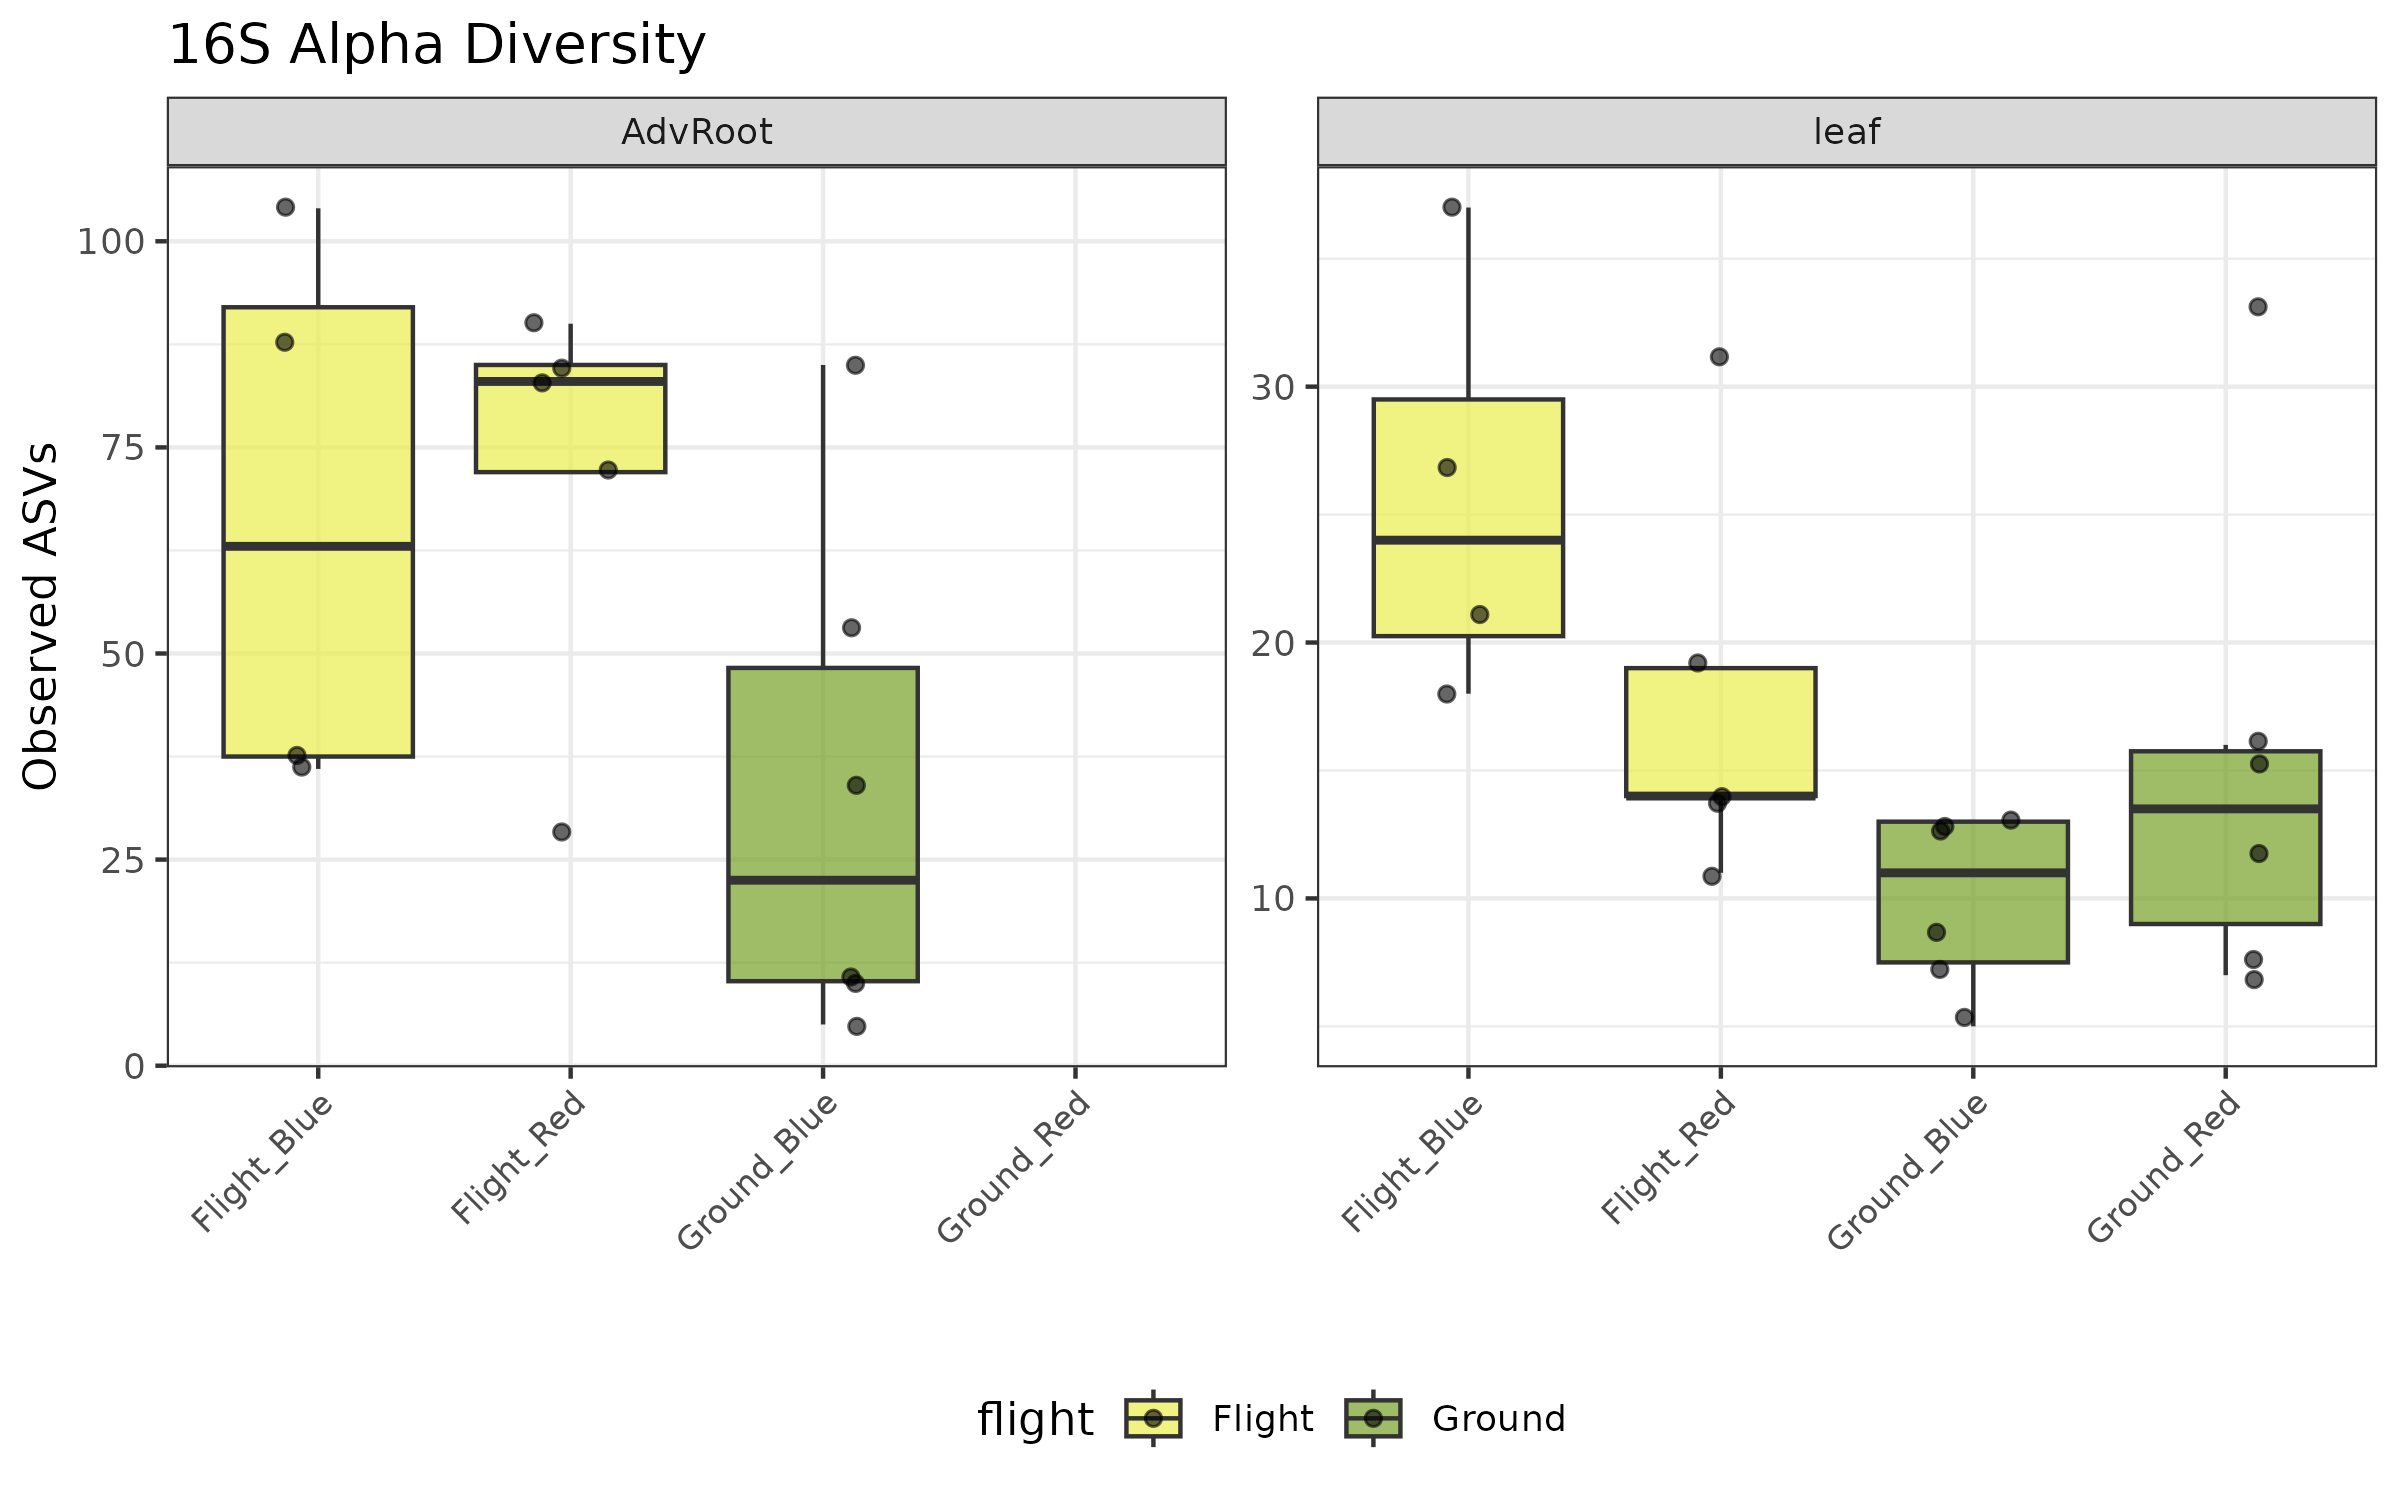
\includegraphics[width=0.8\textwidth]{fig2a_alpha_diversity_16S.png}
\caption{\textbf{Bacterial (16S) alpha diversity} (Observed ASVs) by flight status
and light treatment; flight leaves show higher diversity.}
\label{fig:2a}
\end{figure}

The dysbiosis index quantified community displacement relative to ground controls.
Leaf bacterial communities showed a 2.06-fold increase in dysbiosis during flight
(\(2.06 \pm 0.99\) vs.\ \(1.00 \pm 0.47\); Fig.~\ref{fig:2b16s}). Fungal communities
showed even greater displacement (ITS leaf: \(3.64 \pm 2.78\) vs.\ \(1.00 \pm
0.24\); Fig.~\ref{fig:2bits}), though the PERMANOVA was marginally significant
(\(R^2 = 0.45\), \(p = 0.054\)). Adventitious root fungal communities were
significantly reshaped (\(R^2 = 0.65\), \(F = 8.19\), \(p = 0.001\)).

\begin{figure}[htbp]
\centering
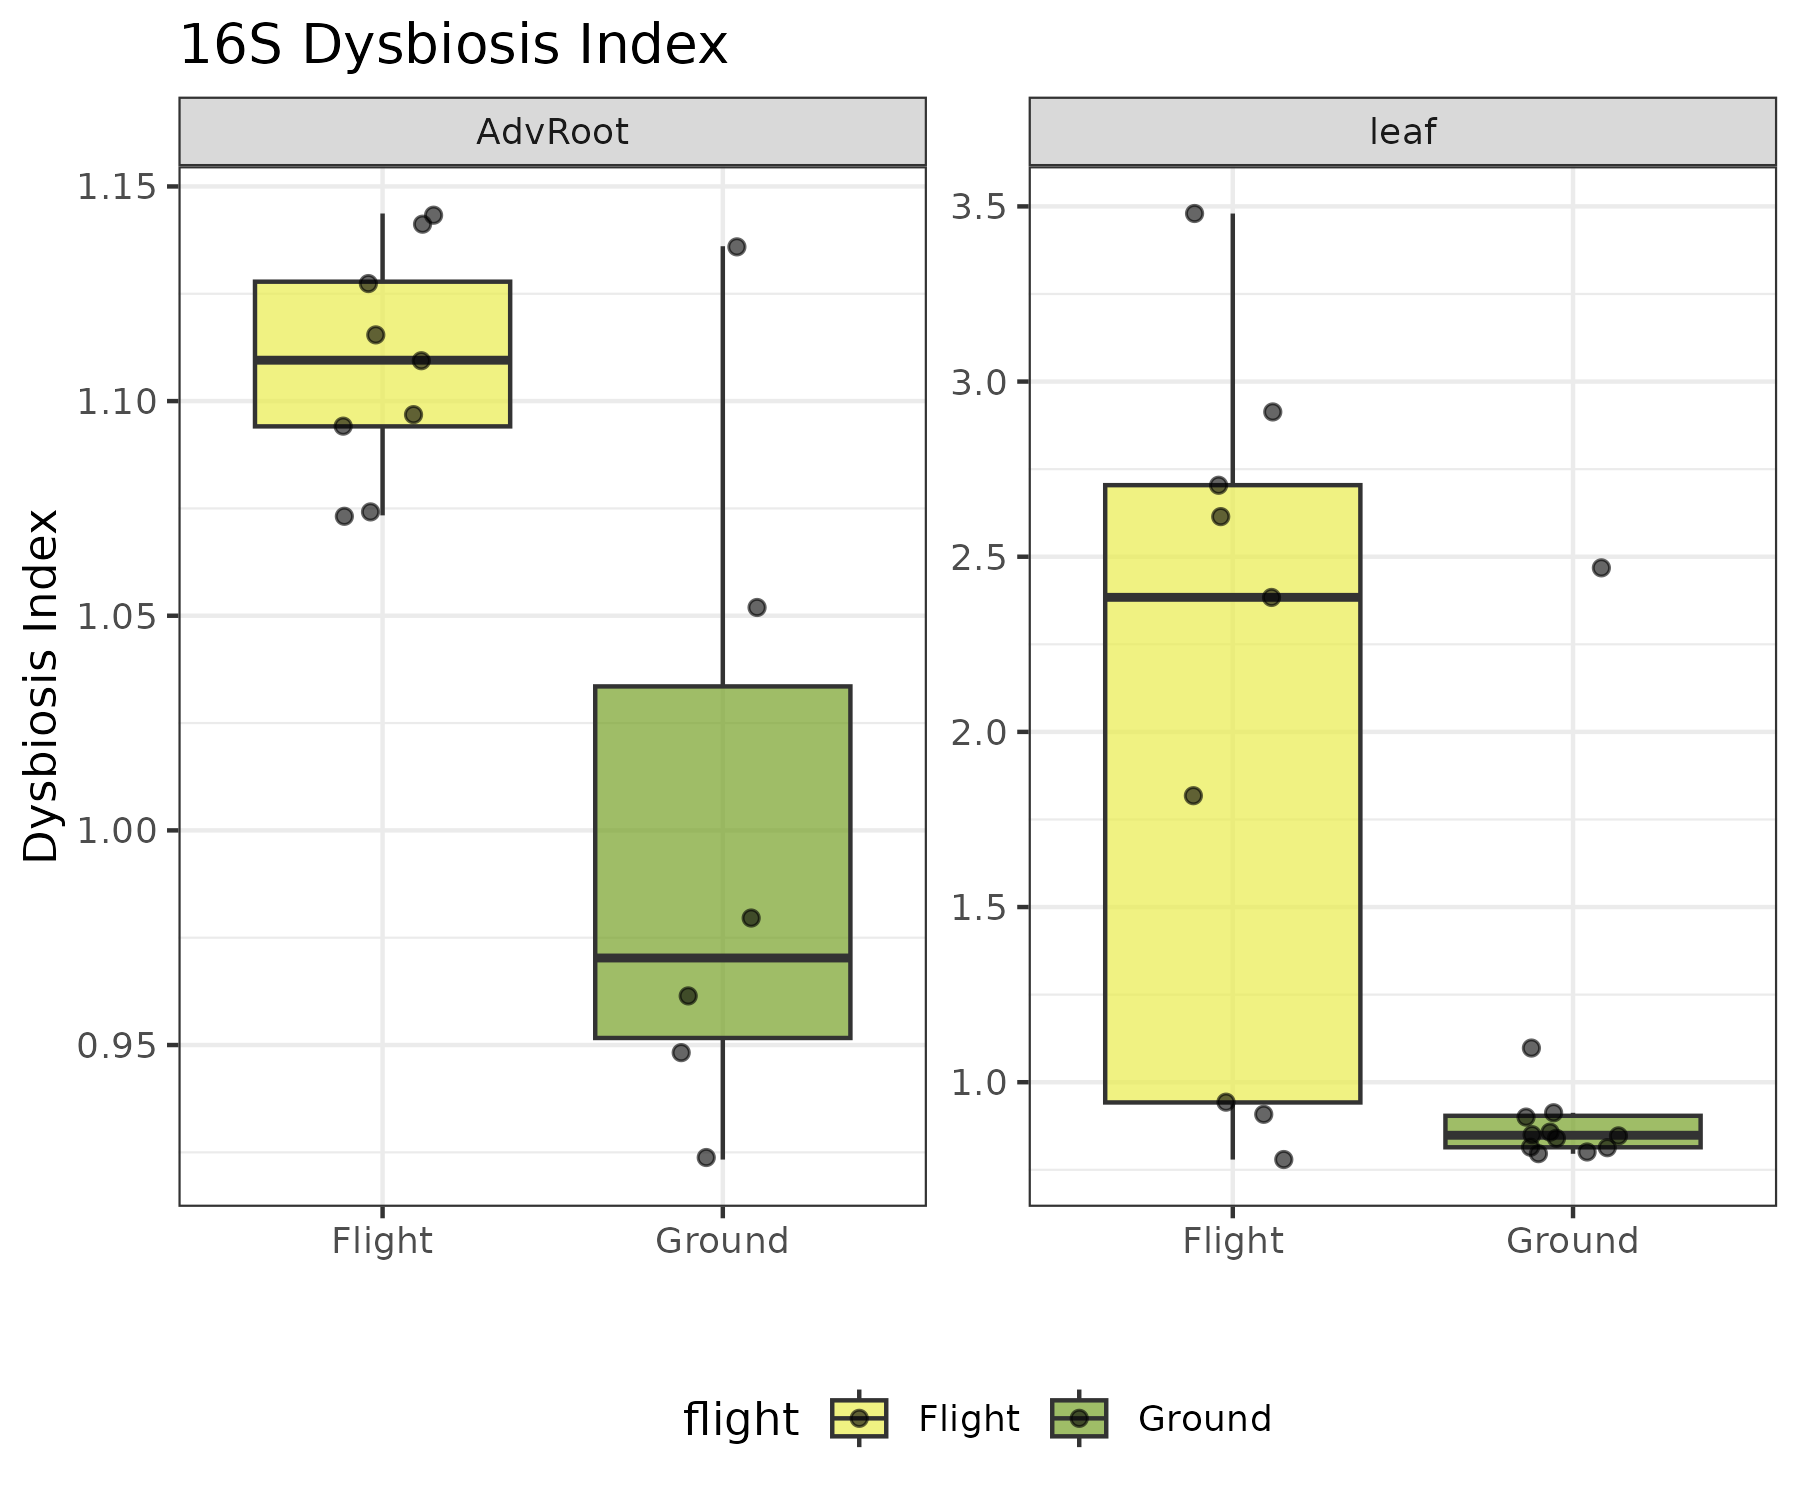
\includegraphics[width=0.48\textwidth]{fig2b_dysbiosis_16S.png}\hfill
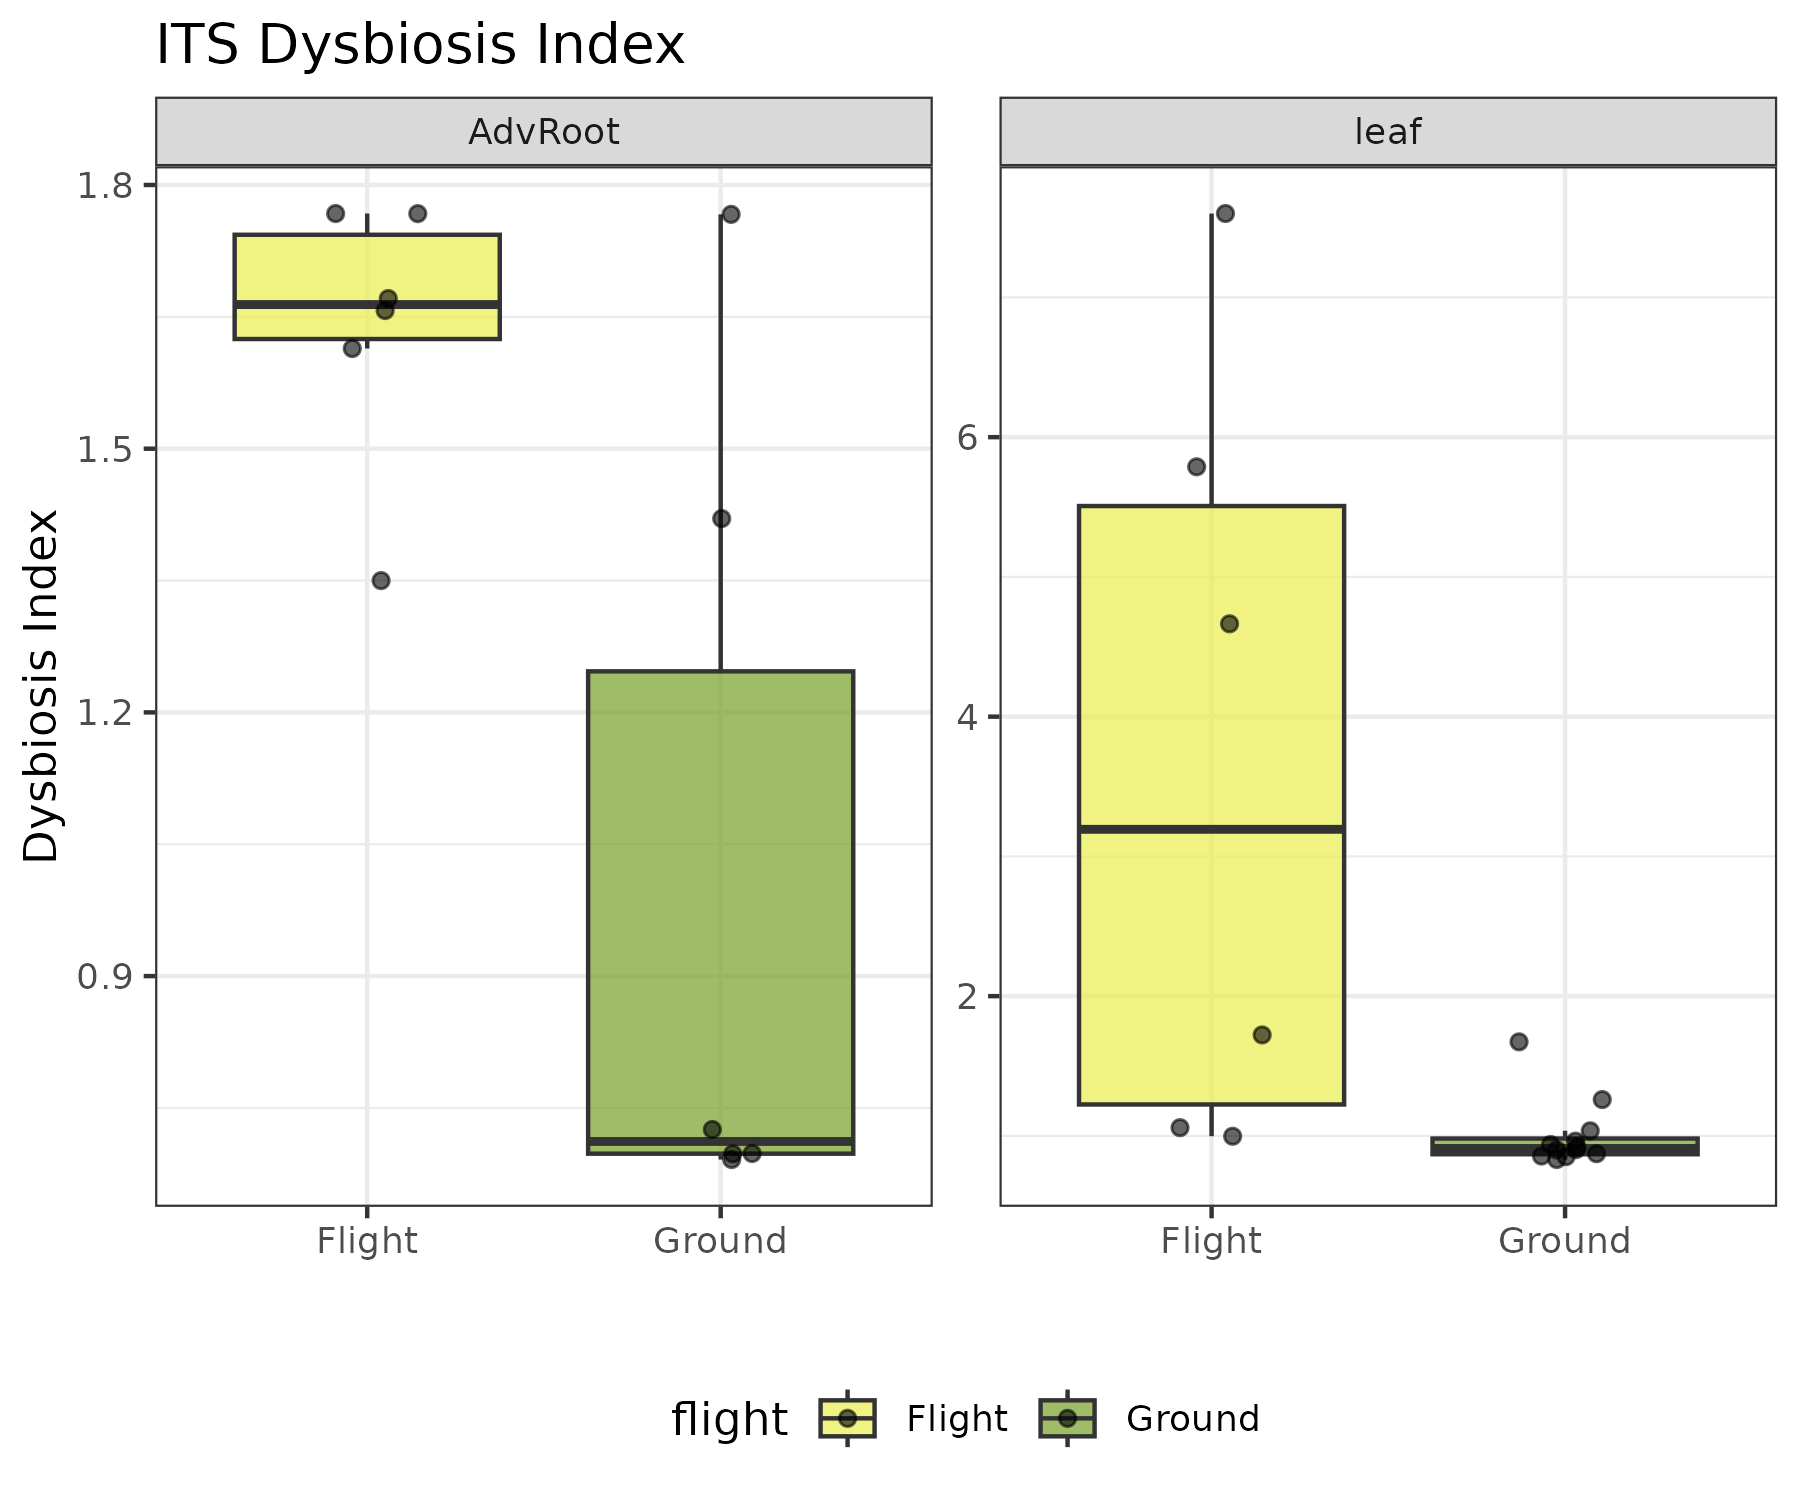
\includegraphics[width=0.48\textwidth]{fig2b_dysbiosis_ITS.png}
\caption{\textbf{Dysbiosis index} (Bray-Curtis displacement from the ground
centroid). Left (16S): bacterial dysbiosis, elevated under flight. Right (ITS):
fungal dysbiosis, largest displacement in flight leaves.}
\label{fig:2b16s}
\end{figure}
\addtocounter{figure}{-1}\refstepcounter{figure}\label{fig:2bits}

ALDEx2 identified few taxa with significant differential abundance under the
conservative dual criterion (\(p < 0.05\) and \(|\text{effect}| > 1\)). In leaf 16S,
\textit{Pantoea} (ASV024) was significantly depleted in flight (effect \(= -1.10\)).
In ITS, \textit{Penicillium citrinum} (ASV003) was significantly depleted in flight
leaves (effect \(= -1.82\)). In adventitious roots, \textit{Fusarium solani} was
significantly depleted in flight (effect \(= -1.82\)).

\subsection{Spaceflight transcriptional response is light-dependent}
DESeq2 analysis revealed a pronounced interaction between spaceflight and light
quality (Table~S2). In leaves, the main flight effect comprised 757 DEGs (404 up,
353 down; Fig.~\ref{fig:3b}), but the flight effect under blue light was nearly
9-fold larger (4{,}716 DEGs) than under red light (523 DEGs) (Fig.~\ref{fig:3}). The
formal interaction term identified 3{,}189 DEGs, confirming that the transcriptional
response to spaceflight is strongly modulated by light quality.

In adventitious roots, the flight response was predominantly upregulation (896 DEGs:
783 up, 113 down, 87\% upregulated; Fig.~\ref{fig:3c}), suggesting activation of
stress response pathways. The interaction was minimal (6 DEGs after shrinkage),
indicating that the root transcriptional response to spaceflight is less
light-dependent than the leaf response.

\begin{figure}[htbp]
\centering
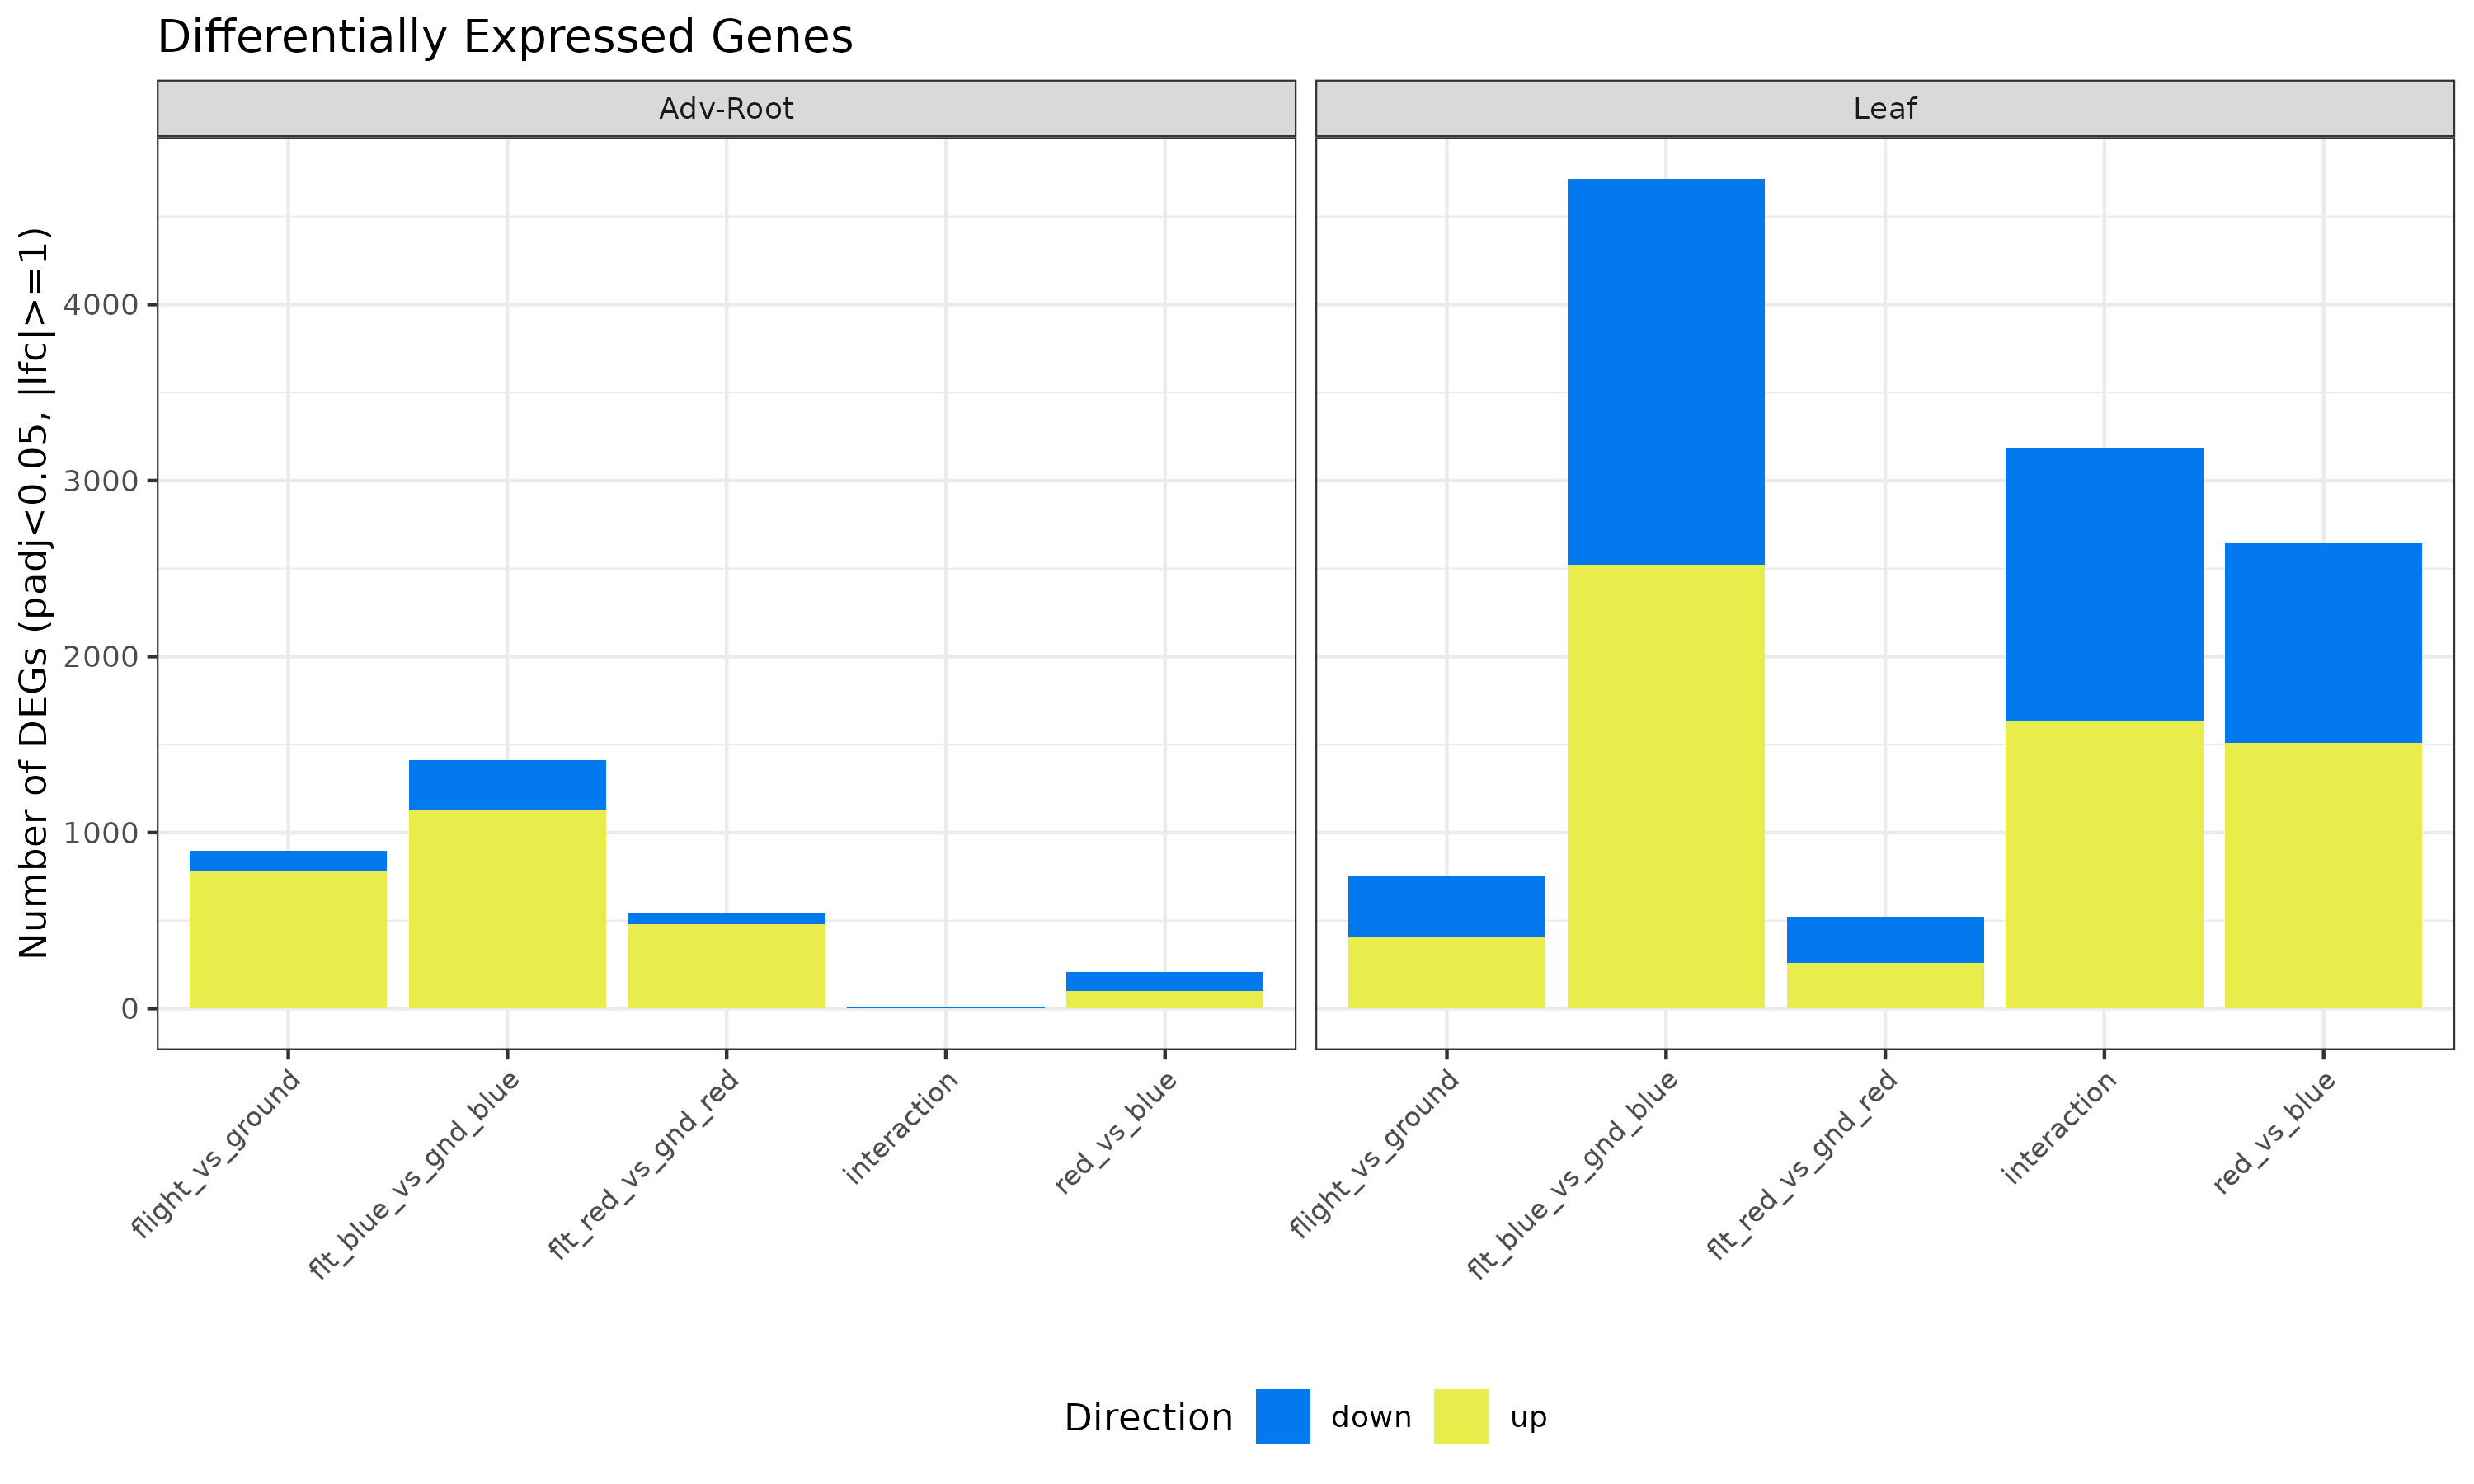
\includegraphics[width=0.8\textwidth]{fig3_deg_summary.png}
\caption{\textbf{DEG summary} across tissue \(\times\) contrast; the leaf blue-light
flight response (4{,}716 DEGs) dwarfs red (523).}
\label{fig:3}
\end{figure}

\begin{figure}[htbp]
\centering
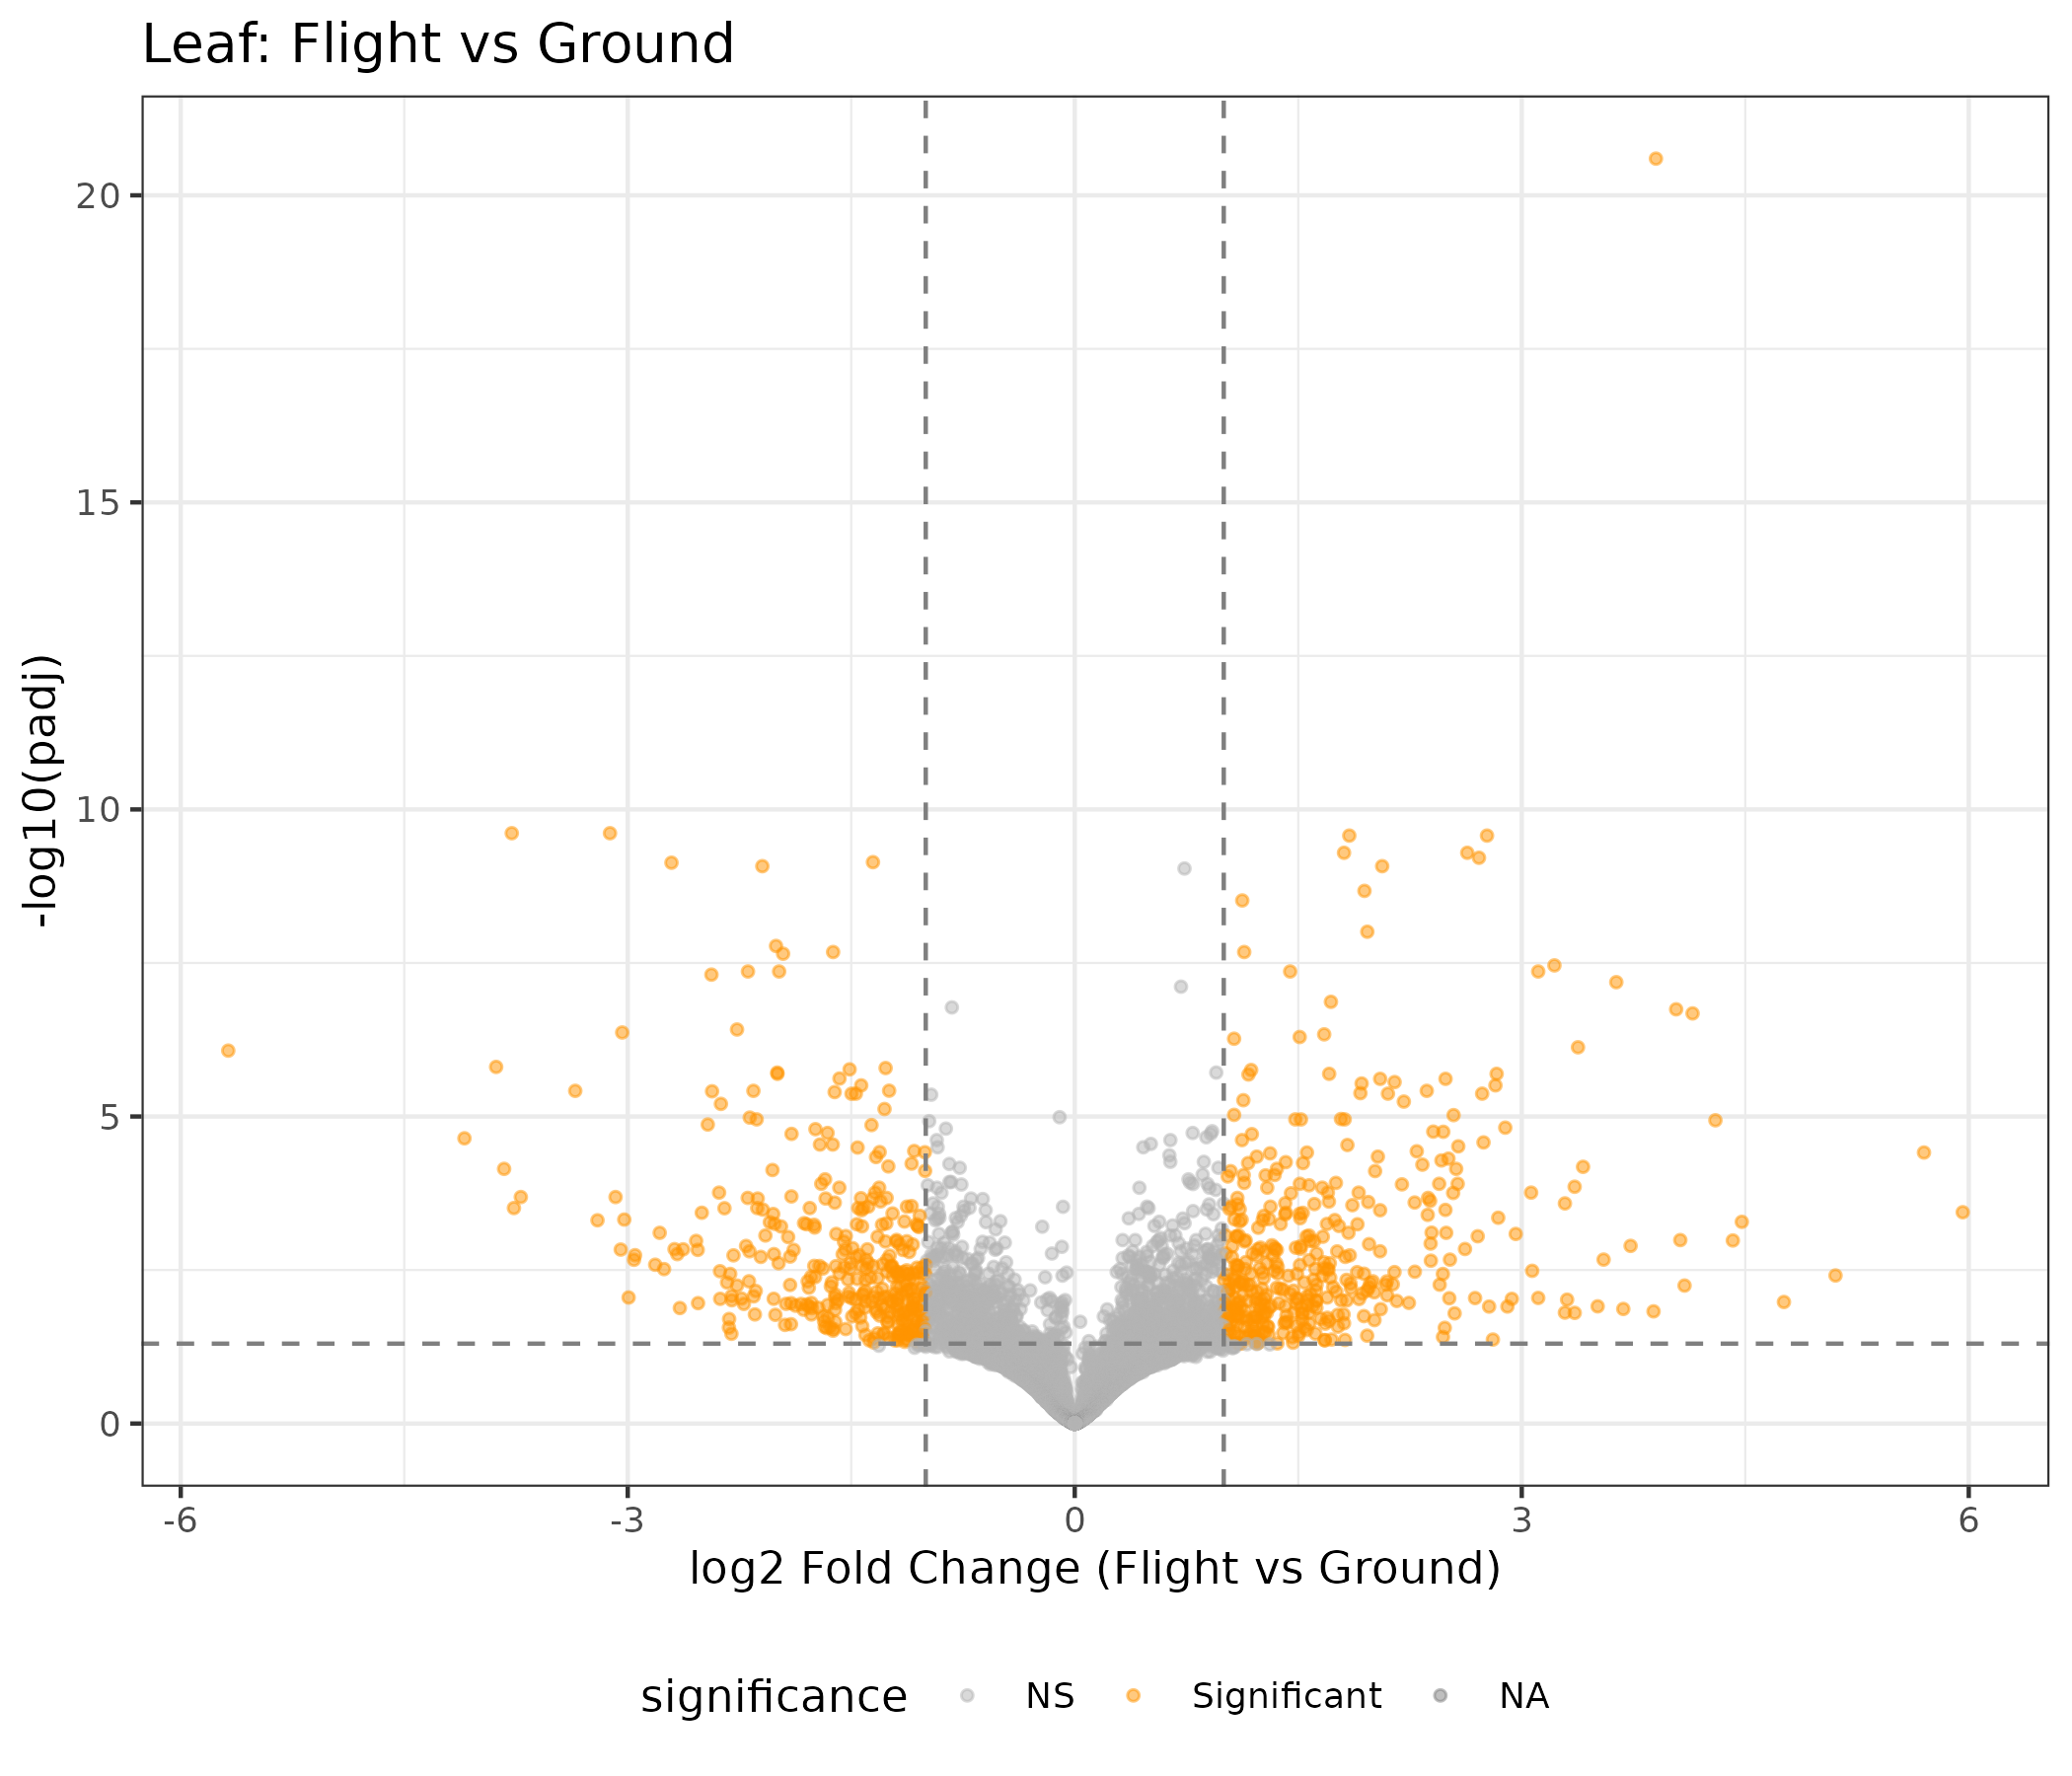
\includegraphics[width=0.48\textwidth]{fig3b_volcano_leaf_flight.png}\hfill
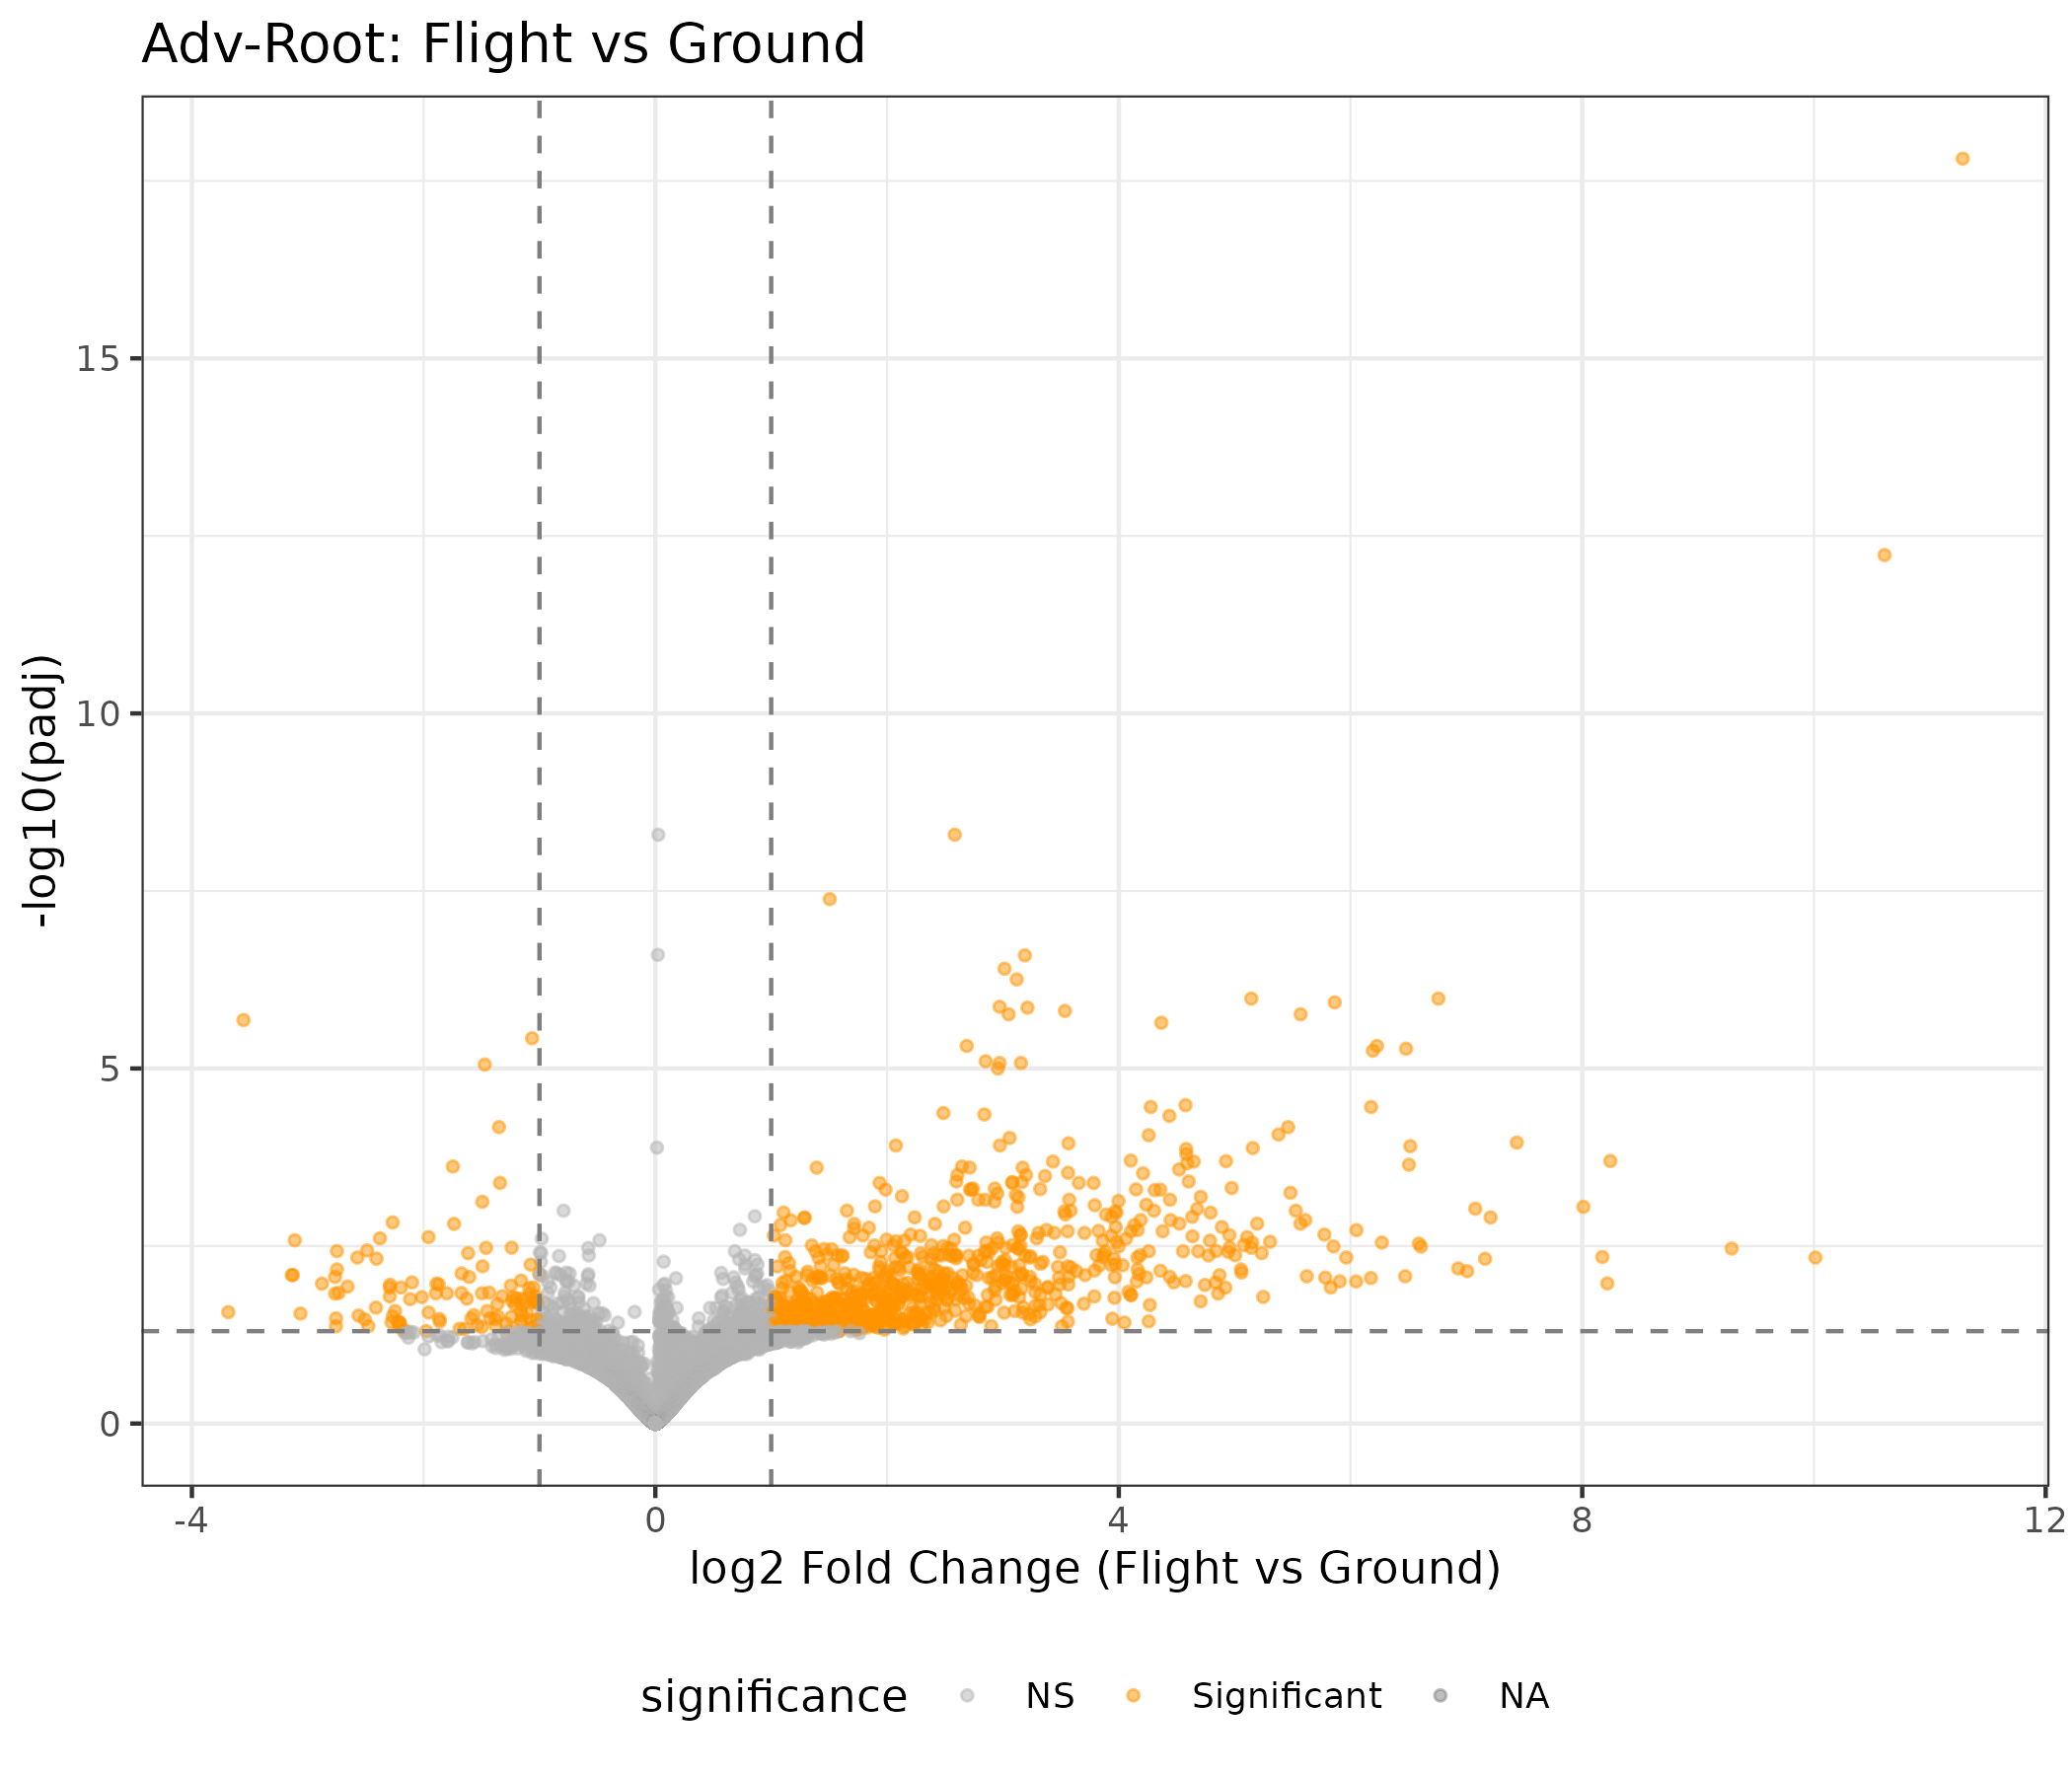
\includegraphics[width=0.48\textwidth]{fig3c_volcano_advroot_flight.png}
\caption{\textbf{Flight-vs-Ground volcano plots.} Left (\(3B\)): leaf. Right
(\(3C\)): adventitious root (predominantly upregulation).}
\label{fig:3b}
\end{figure}
\addtocounter{figure}{-1}\refstepcounter{figure}\label{fig:3c}

\subsection{WGCNA identifies a microbe-driven host transcriptional module}
WGCNA of the leaf transcriptome identified 13 modules (power = 20;
Fig.~\ref{fig:4leaf}), with the turquoise module (\(n = 2{,}037\) genes) showing the
strongest flight correlation (\(r = +0.73\), \(p_{\mathrm{adj}} = 0.001\)) and the
blue module (\(n = 1{,}012\)) the strongest anti-correlation (\(r = -0.79\),
\(p_{\mathrm{adj}} = 3\times10^{-4}\)). Four leaf modules were classified as
co-regulated (correlated with both flight and dysbiosis; Table~S5).

In adventitious roots, WGCNA identified 17 modules (power = 18). The key finding was
the black module (\(n = 169\) genes), strongly correlated with ITS dysbiosis (\(r =
-0.85\), \(p_{\mathrm{adj}} = 0.001\)) but not with flight status (\(r = -0.38\),
\(p = 0.32\); Fig.~\ref{fig:4advroot}). This module was classified as
microbe-driven, representing a host transcriptional response to fungal community
changes independent of the direct spaceflight stimulus. GO enrichment of the black
module itself was limited --- its only significantly enriched term was the cellular
component ``nucleus'' --- so it is defined here by its microbe-driven trait
association; the adventitious-root oxidative-stress program was instead concentrated
in the larger turquoise module (see below).

GO enrichment of all modules revealed biologically coherent signatures (Table~S10).
In leaves, the black module was enriched for photosynthesis and photosystem genes
(\(p_{\mathrm{adj}} = 4.4\times10^{-25}\)), while the red module was enriched for RNA
binding and protein binding. In adventitious roots, the turquoise module (the
largest, \(n = 1{,}768\)) was enriched for oxidative stress response (peroxidase
activity, \(p_{\mathrm{adj}} = 4.2\times10^{-9}\); hydrogen peroxide catabolism,
\(p_{\mathrm{adj}} = 1.1\times10^{-8}\); glutathione transferase activity,
\(p_{\mathrm{adj}} = 3.9\times10^{-7}\)), consistent with spaceflight-induced
oxidative stress.

\begin{figure}[htbp]
\centering

\includegraphics[width=0.48\textwidth]{fig4_module_traits_Leaf.png}\hfill
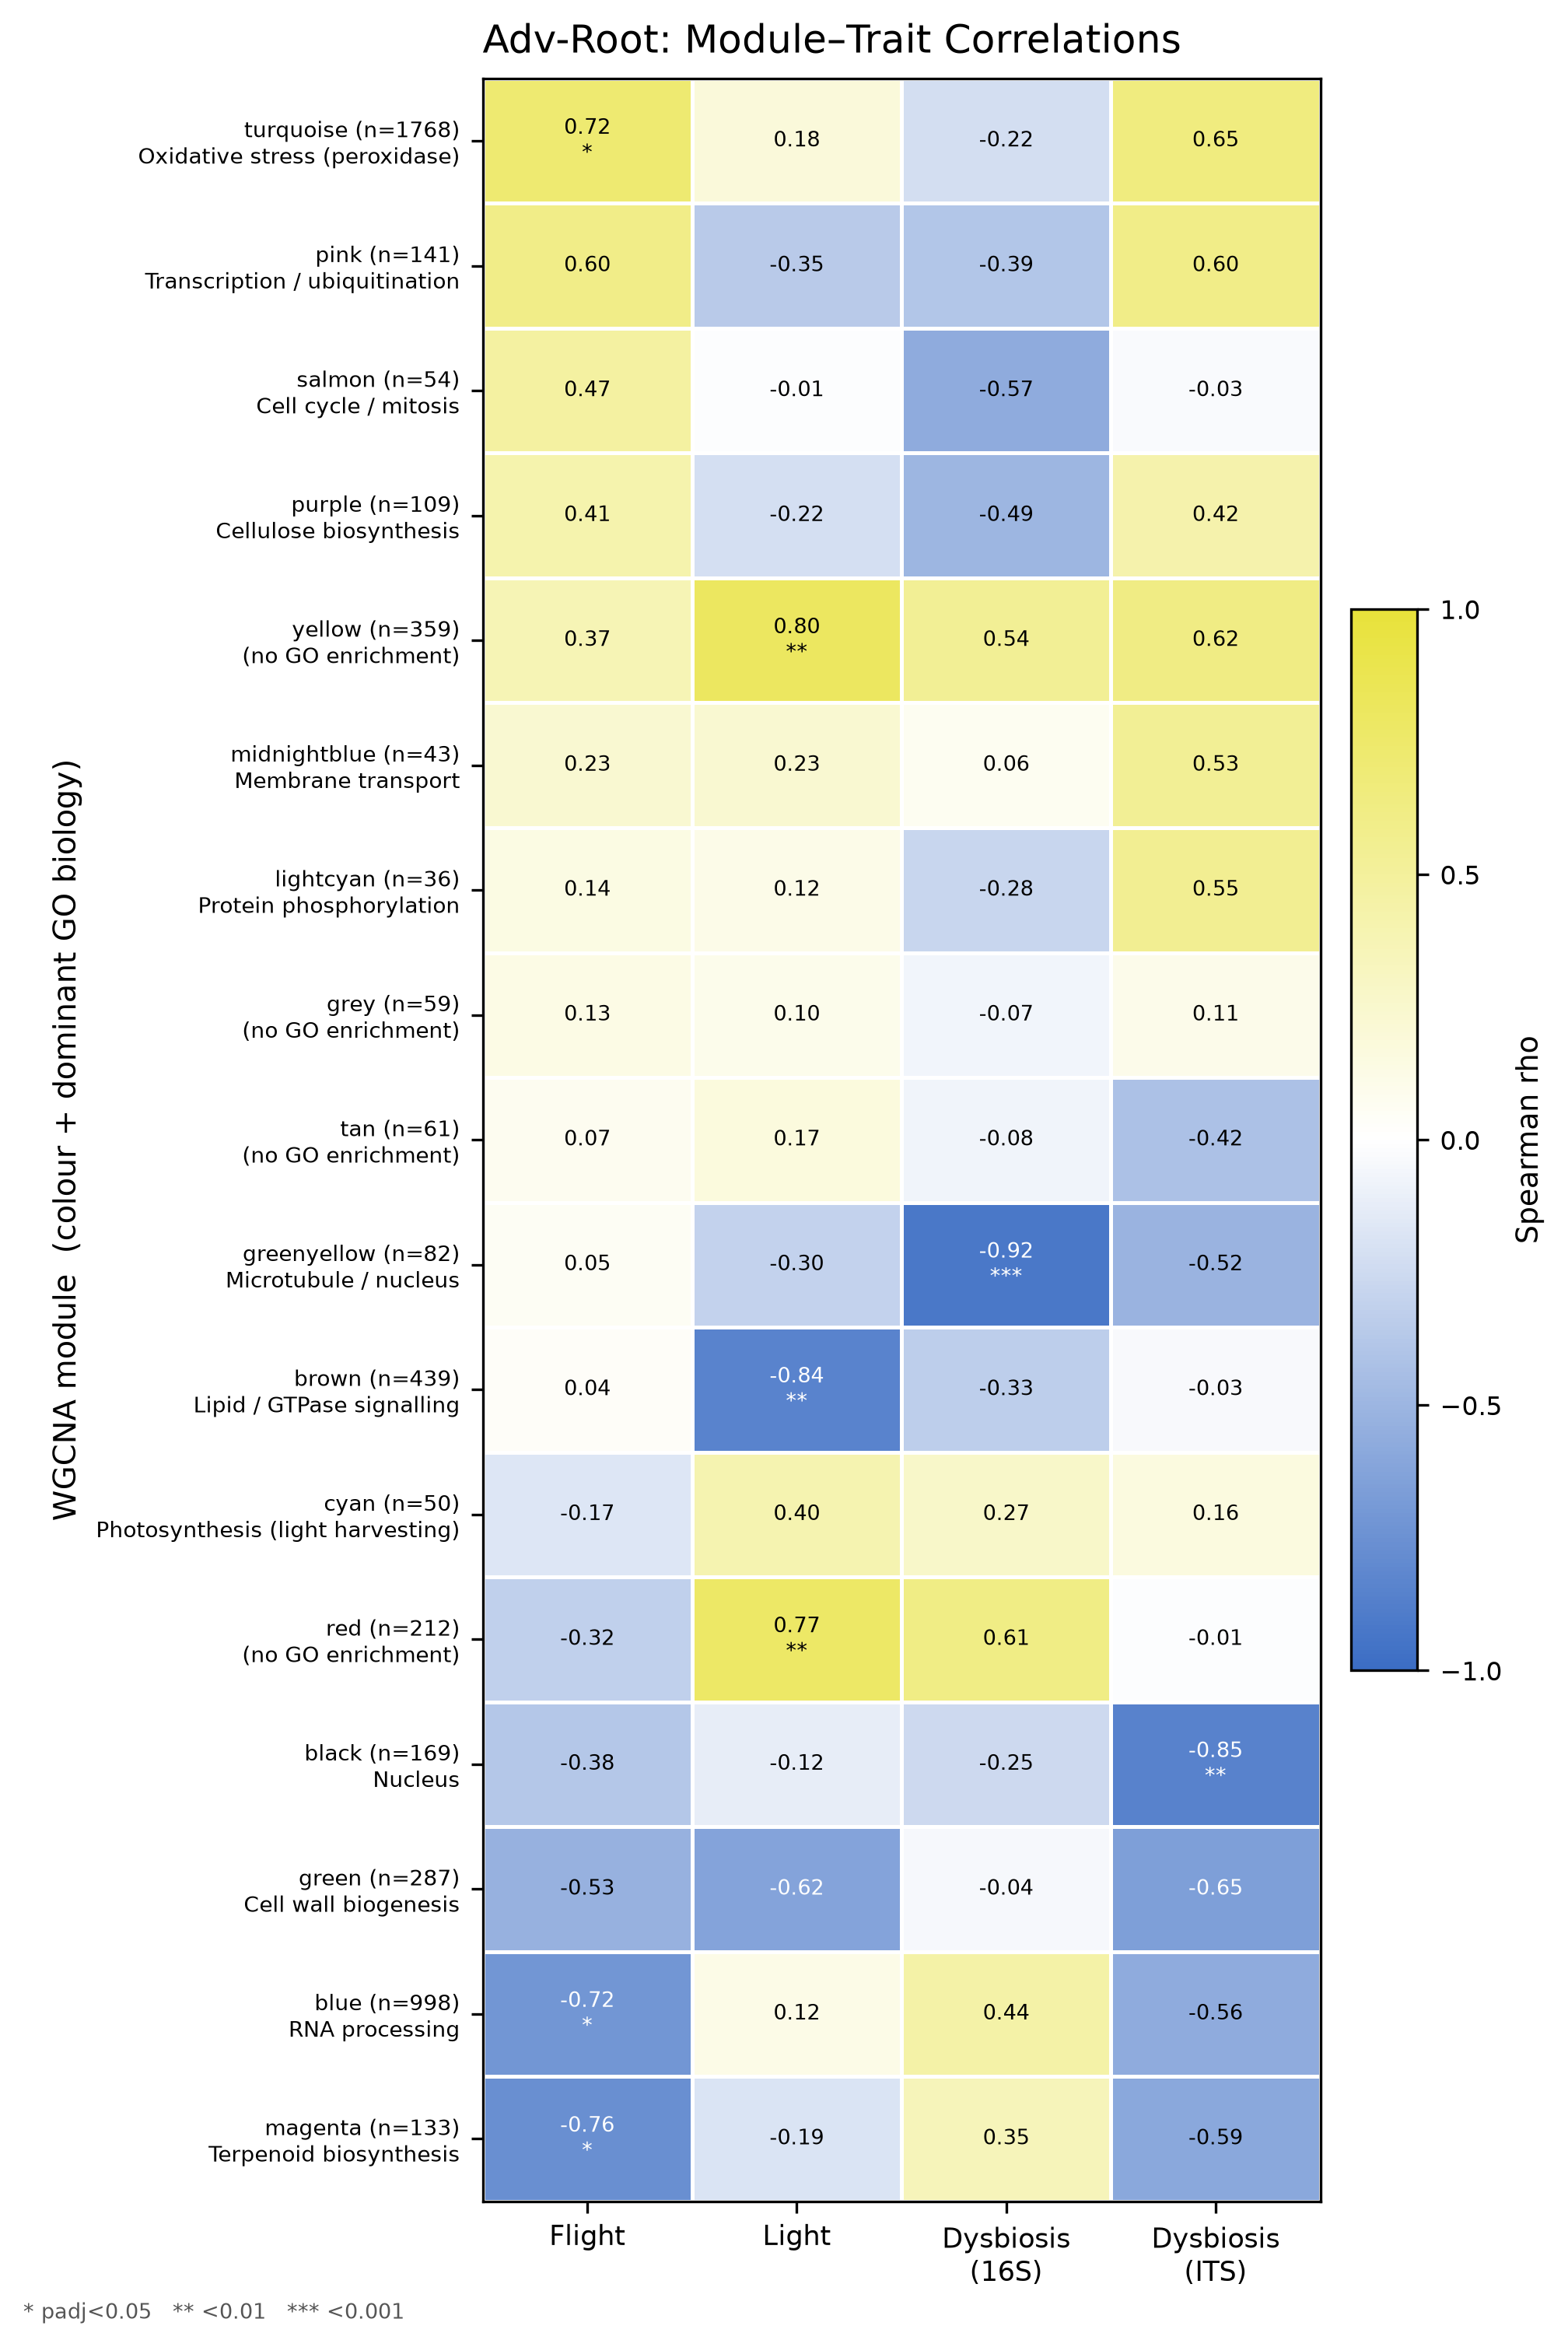
\includegraphics[width=0.48\textwidth]{fig4_module_traits_AdvRoot.png}
\caption{\textbf{WGCNA module--trait correlations} (flight, light, 16S/ITS
dysbiosis). Left: leaf. Right: adventitious root --- the black (nucleus) module
tracks ITS dysbiosis (\(r = -0.85\)) but not flight; the turquoise
(oxidative-stress/peroxidase) module is the largest flight-correlated module. Each
module is labelled with its dominant GO biology (Table~\ref{tab:go}).}
\label{fig:4leaf}
\end{figure}
\addtocounter{figure}{-1}\refstepcounter{figure}\label{fig:4advroot}

\subsection{Module functional annotation (GO)}
To make the WGCNA module colours interpretable, each module was annotated with its
dominant biology from per-module Gene Ontology enrichment
(Table~\ref{tab:go}). These human-readable labels are shown alongside the module
colours on the axes of Figs~\ref{fig:4leaf} and \ref{fig:6}. Modules with no
significant enrichment are marked accordingly.

\begin{longtable}{@{}l l p{5.6cm}@{}}
\caption{GO-based functional annotation of WGCNA modules.}\label{tab:go}\\
\toprule
\textbf{Tissue / Module} & \textbf{GO biology (dominant)} & \textbf{Representative GO terms} \\
\midrule
\endfirsthead
\multicolumn{3}{c}{\tablename\ \thetable\ --- continued}\\
\toprule
\textbf{Tissue / Module} & \textbf{GO biology (dominant)} & \textbf{Representative GO terms} \\
\midrule
\endhead
\bottomrule
\endfoot
Adv-Root / black & Nucleus & nucleus \\
Adv-Root / blue & RNA processing & protein binding; RNA binding; RNA modification \\
Adv-Root / brown & Lipid / GTPase signalling & ATP-dependent diacylglycerol kinase activity; phospholipase C-activati\ldots \\
Adv-Root / cyan & Photosynthesis (light harvesting) & photosynthesis, light harvesting; photosynthesis; photosystem I \\
Adv-Root / green & Cell wall biogenesis & xyloglucan metabolic process; cell wall; xyloglucan:xyloglucosyl trans\ldots \\
Adv-Root / greenyellow & Microtubule / nucleus & microtubule binding; ATP binding; nucleus \\
Adv-Root / lightcyan & Protein phosphorylation & protein phosphorylation; protein kinase activity; ATP binding \\
Adv-Root / magenta & Terpenoid biosynthesis & acyltransferase activity; terpene synthase activity; terpenoid biosynt\ldots \\
Adv-Root / midnightblue & Membrane transport & transmembrane transporter activity; transmembrane transport; membrane \\
Adv-Root / pink & Transcription / ubiquitination & DNA-binding transcription factor activity; ubiquitin protein ligase ac\ldots \\
Adv-Root / purple & Cellulose biosynthesis & cellulose synthase (UDP-forming) activity; cellulose biosynthetic proc\ldots \\
Adv-Root / salmon & Cell cycle / mitosis & cyclin-dependent protein serine/threonine kinase regulator activity; m\ldots \\
Adv-Root / turquoise & Oxidative stress (peroxidase) & peroxidase activity; hydrogen peroxide catabolic process; heme binding \\
Leaf / black & Photosynthesis \& ribosome & photosynthesis; ribosome; photosystem I \\
Leaf / blue & Phosphate starvation / transport & DNA-binding transcription factor activity; cellular response to phosph\ldots \\
Leaf / brown & Lignin / phenolic metabolism & heme binding; endopeptidase inhibitor activity; cation binding \\
Leaf / green & Protein ubiquitination & protein ubiquitination; ubiquitin-protein transferase activity; cell s\ldots \\
Leaf / greenyellow & Chitinase / defense & chitinase activity; chitin catabolic process; chitin binding \\
Leaf / magenta & Transcription / ethylene & regulation of DNA-templated transcription; ethylene-activated signalin\ldots \\
Leaf / pink & Cell wall / glucan & cell wall; xyloglucan:xyloglucosyl transferase activity; glucan metabo\ldots \\
Leaf / purple & Fe--S cluster / biosynthesis & iron-sulfur cluster binding; biosynthetic process \\
Leaf / red & RNA processing & RNA binding; protein binding; RNA modification \\
Leaf / tan & Oxidative stress (peroxidase) & hydrogen peroxide catabolic process; peroxidase activity; response to\ldots \\
Leaf / turquoise & Chromatin / nucleosome & nucleosome; structural constituent of chromatin; microtubule binding \\
\end{longtable}

\subsection{MOFA+ confirms dominant flight factor and cross-omics coordination}
MOFA+ integration of 21 matched leaf samples across three omics views
(transcriptome: 2{,}000 genes; 16S: 348 ASVs; ITS: 77 ASVs) identified 5 factors.
Factor 1 was the dominant signal, explaining 48.0\% of transcriptome variance, 12.0\%
of 16S variance, and 3.0\% of ITS variance (Fig.~\ref{fig:5a}). Factor 1 was
significantly correlated with flight status (Spearman \(\rho = -0.76\),
\(p_{\mathrm{adj}} = 0.001\); Fig.~\ref{fig:5b}), confirming that spaceflight is the
primary axis of coordinated variation across omics layers. Factor 2 trended with 16S
dysbiosis (\(\rho = -0.52\), \(p = 0.018\), \(p_{\mathrm{adj}} = 0.089\)), while
Factor 3 trended with both light treatment (\(\rho = 0.52\)) and ITS dysbiosis
(\(\rho = 0.50\)). The transcriptome contributed the highest-weighted features to
all factors, but microbial features were consistently present in the top weights
(Table~S8).

\begin{figure}[htbp]
\centering
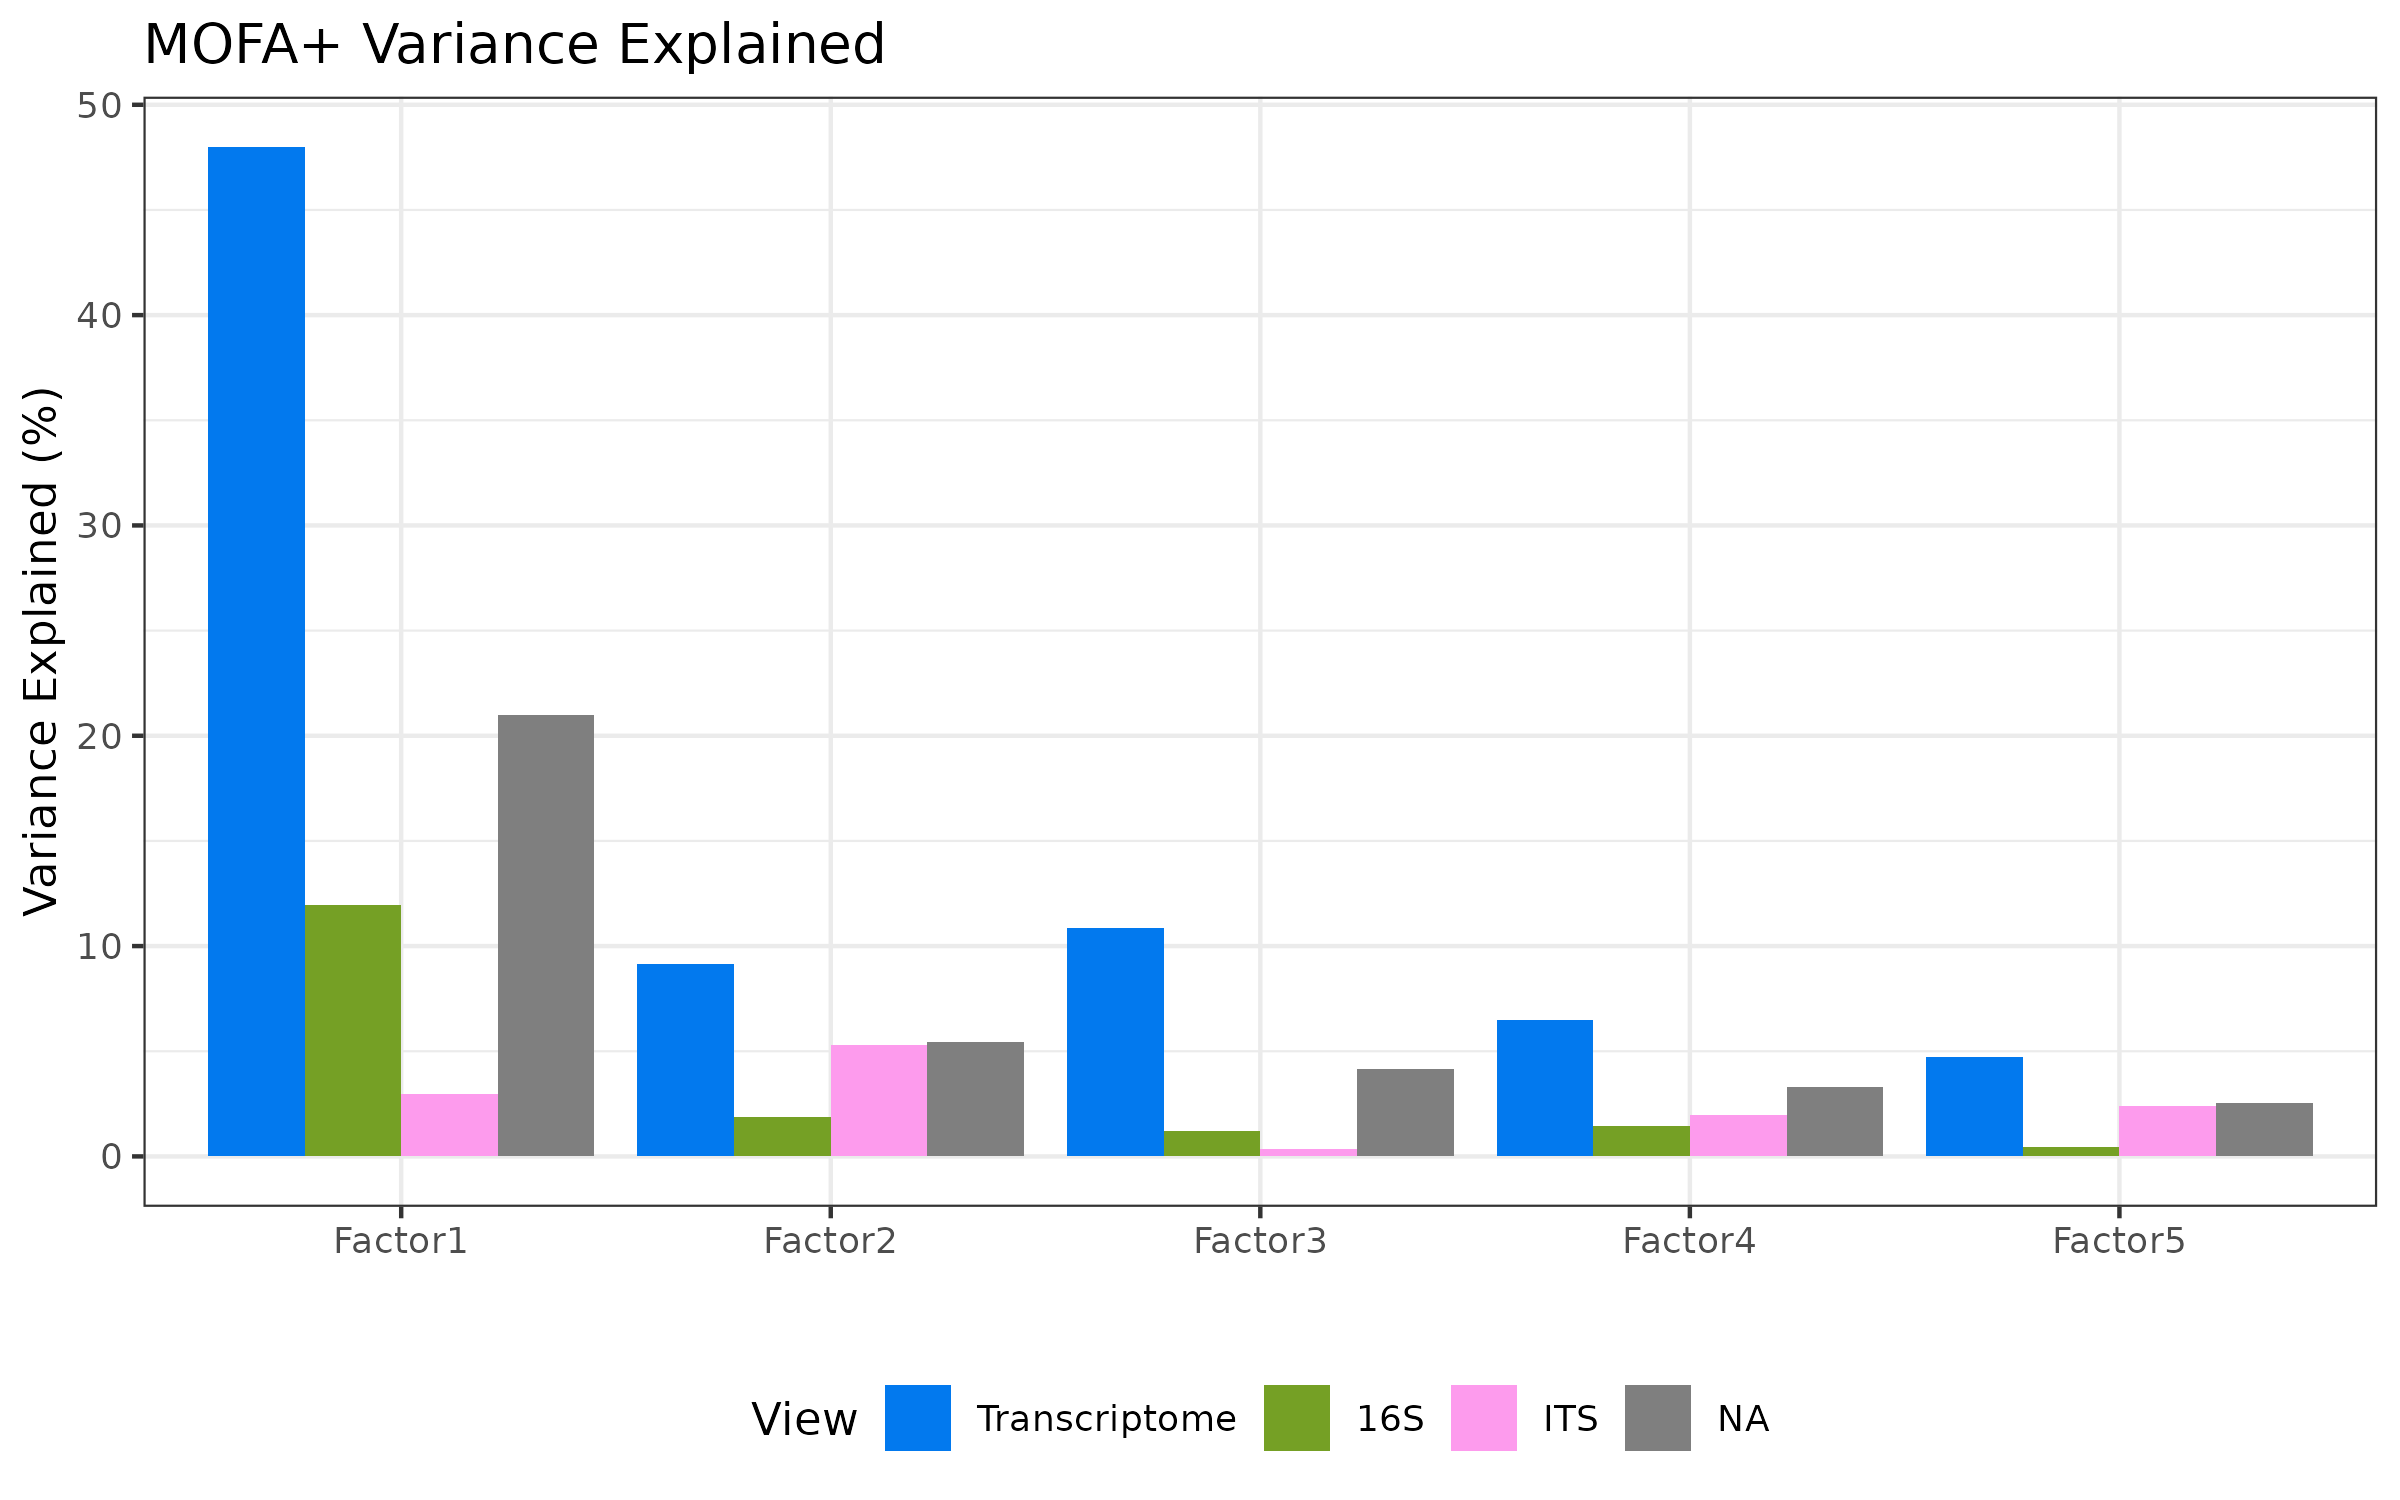
\includegraphics[width=0.48\textwidth]{fig5a_mofa_variance.png}\hfill
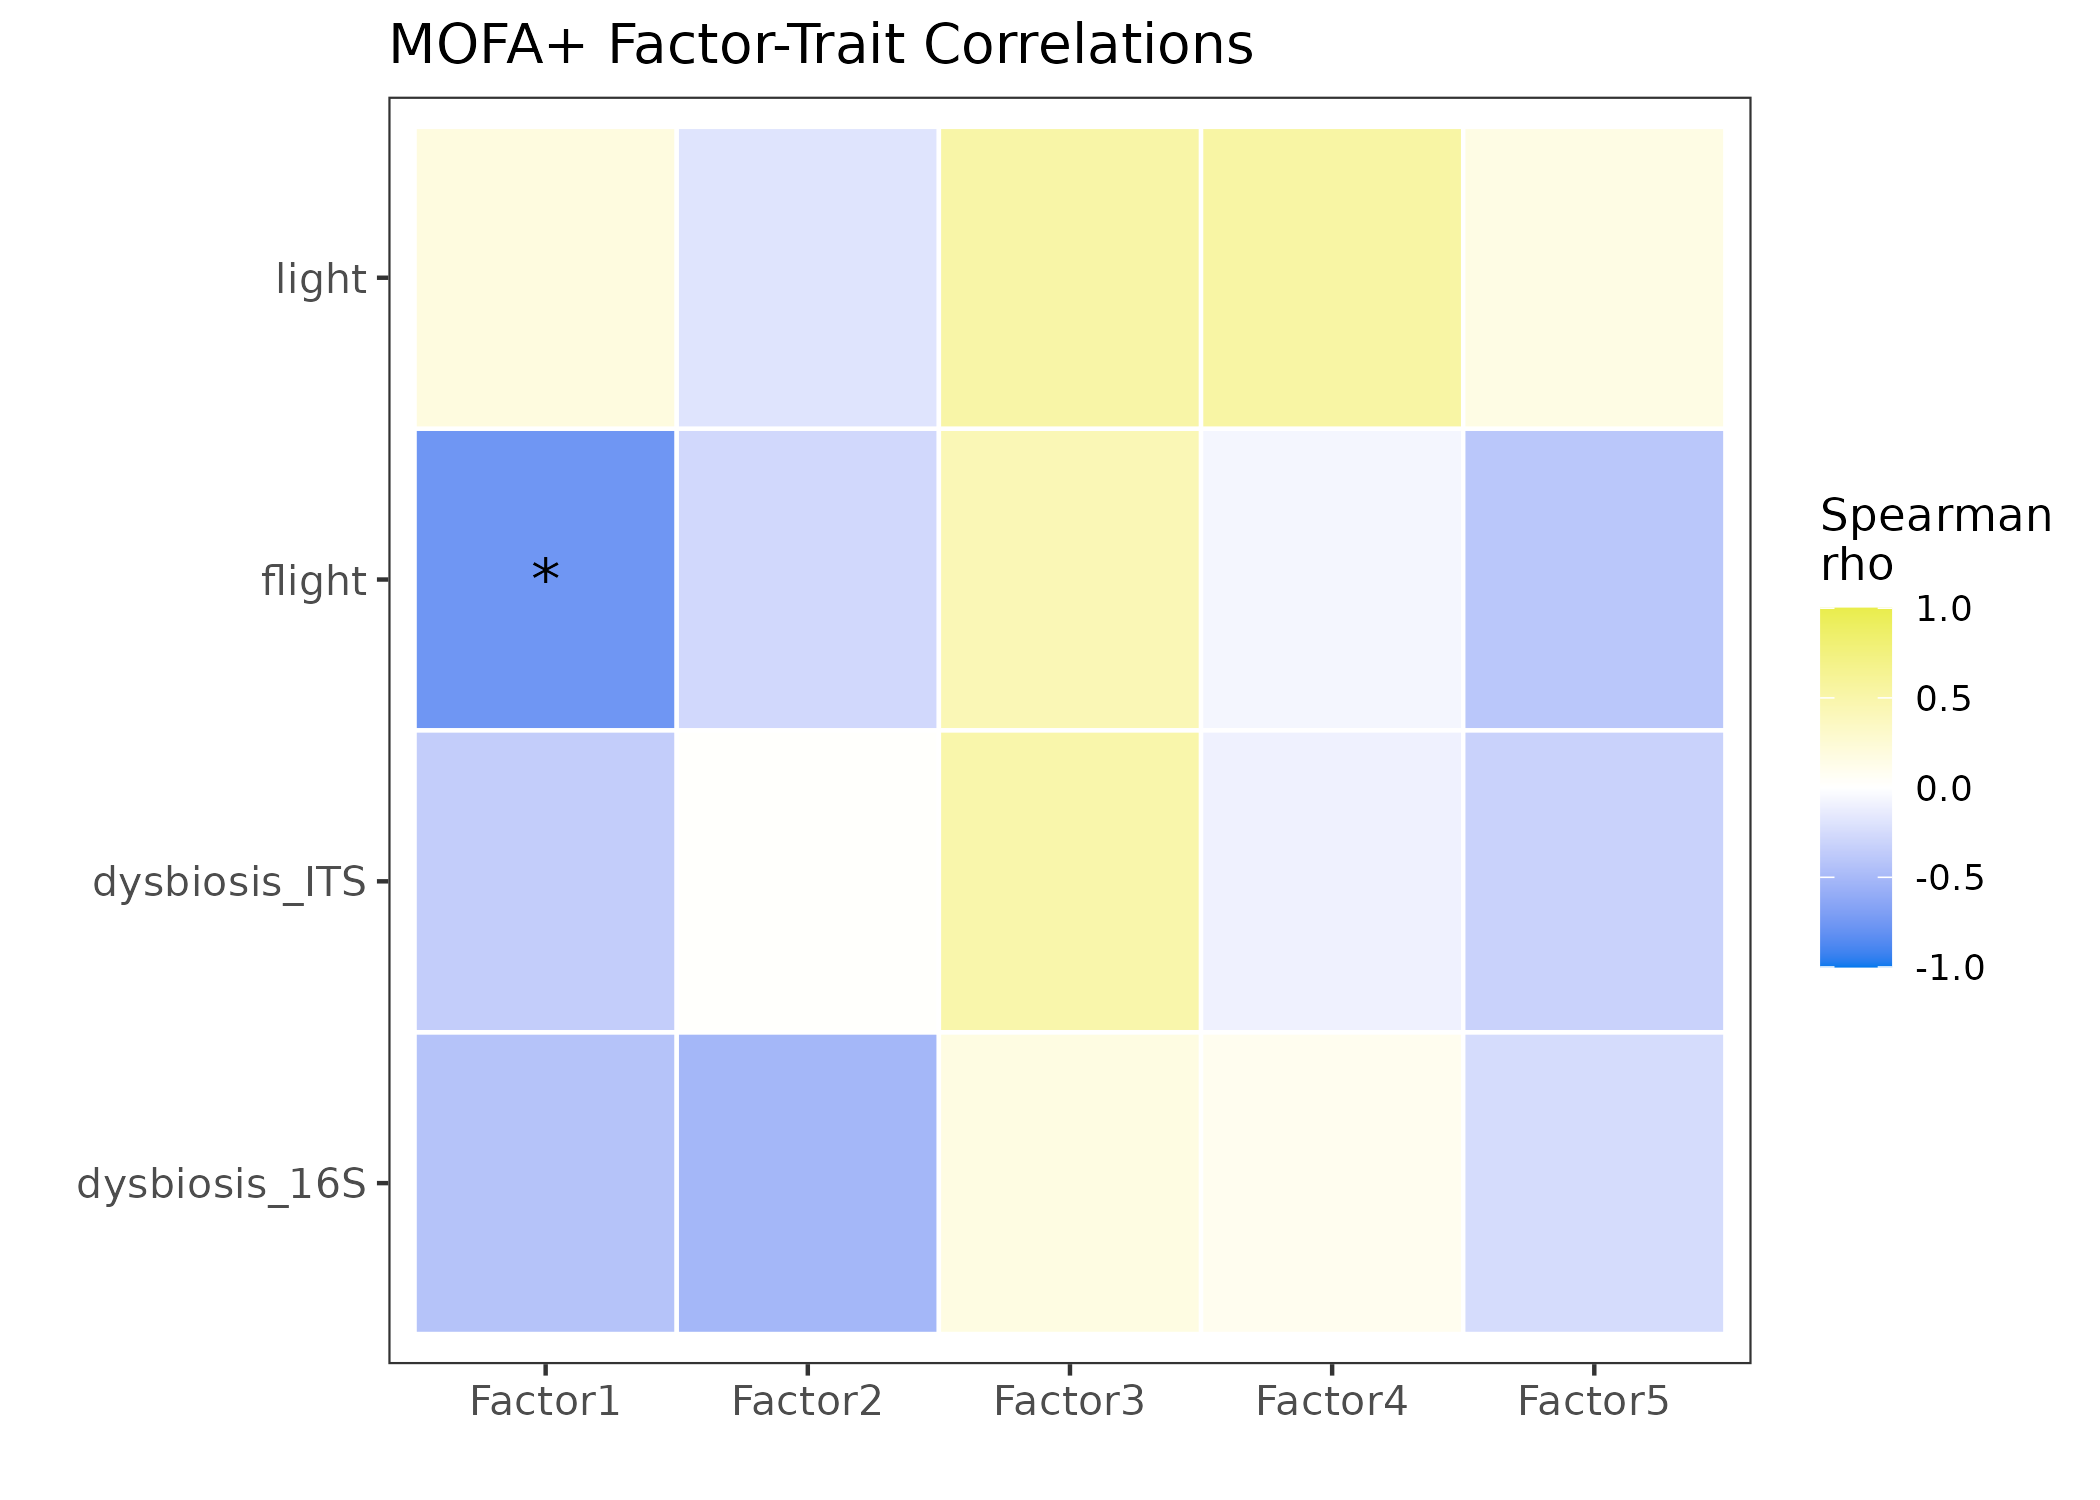
\includegraphics[width=0.48\textwidth]{fig5b_mofa_correlations.png}
\caption{\textbf{MOFA+ integration.} Left (\(5A\)): variance explained per factor per
view. Right (\(5B\)): factor--trait correlations; Factor 1 captures flight (\(\rho =
-0.76\)).}
\label{fig:5a}
\end{figure}
\addtocounter{figure}{-1}\refstepcounter{figure}\label{fig:5b}

\subsection{Module-taxon correlations link host modules to specific bacteria}
Bipartite correlation networks identified 29 significant module-taxon relationships
(BH \(p_{\mathrm{adj}} < 0.05\)), predominantly in leaf 16S (28 of 29;
Fig.~\ref{fig:6}; Table~S9). The flight-associated turquoise module positively
correlated with \textit{Methylobacterium-Methylorubrum} (\(\rho = +0.76\),
\(p_{\mathrm{adj}} = 0.001\)), \textit{Burkholderia-Caballeronia-Paraburkholderia}
(\(\rho = +0.74\), \(p_{\mathrm{adj}} = 0.003\)), and \textit{Azospirillum} (\(\rho =
+0.68\), \(p_{\mathrm{adj}} = 0.012\)) --- all genera associated with plant growth
promotion and nitrogen fixation. The anti-correlated blue module showed the inverse
pattern. The brown module correlated negatively with \textit{Pantoea} (\(\rho =
-0.79\)) and \textit{Paenibacillus} (\(\rho = -0.77\)).

\begin{figure}[htbp]
\centering
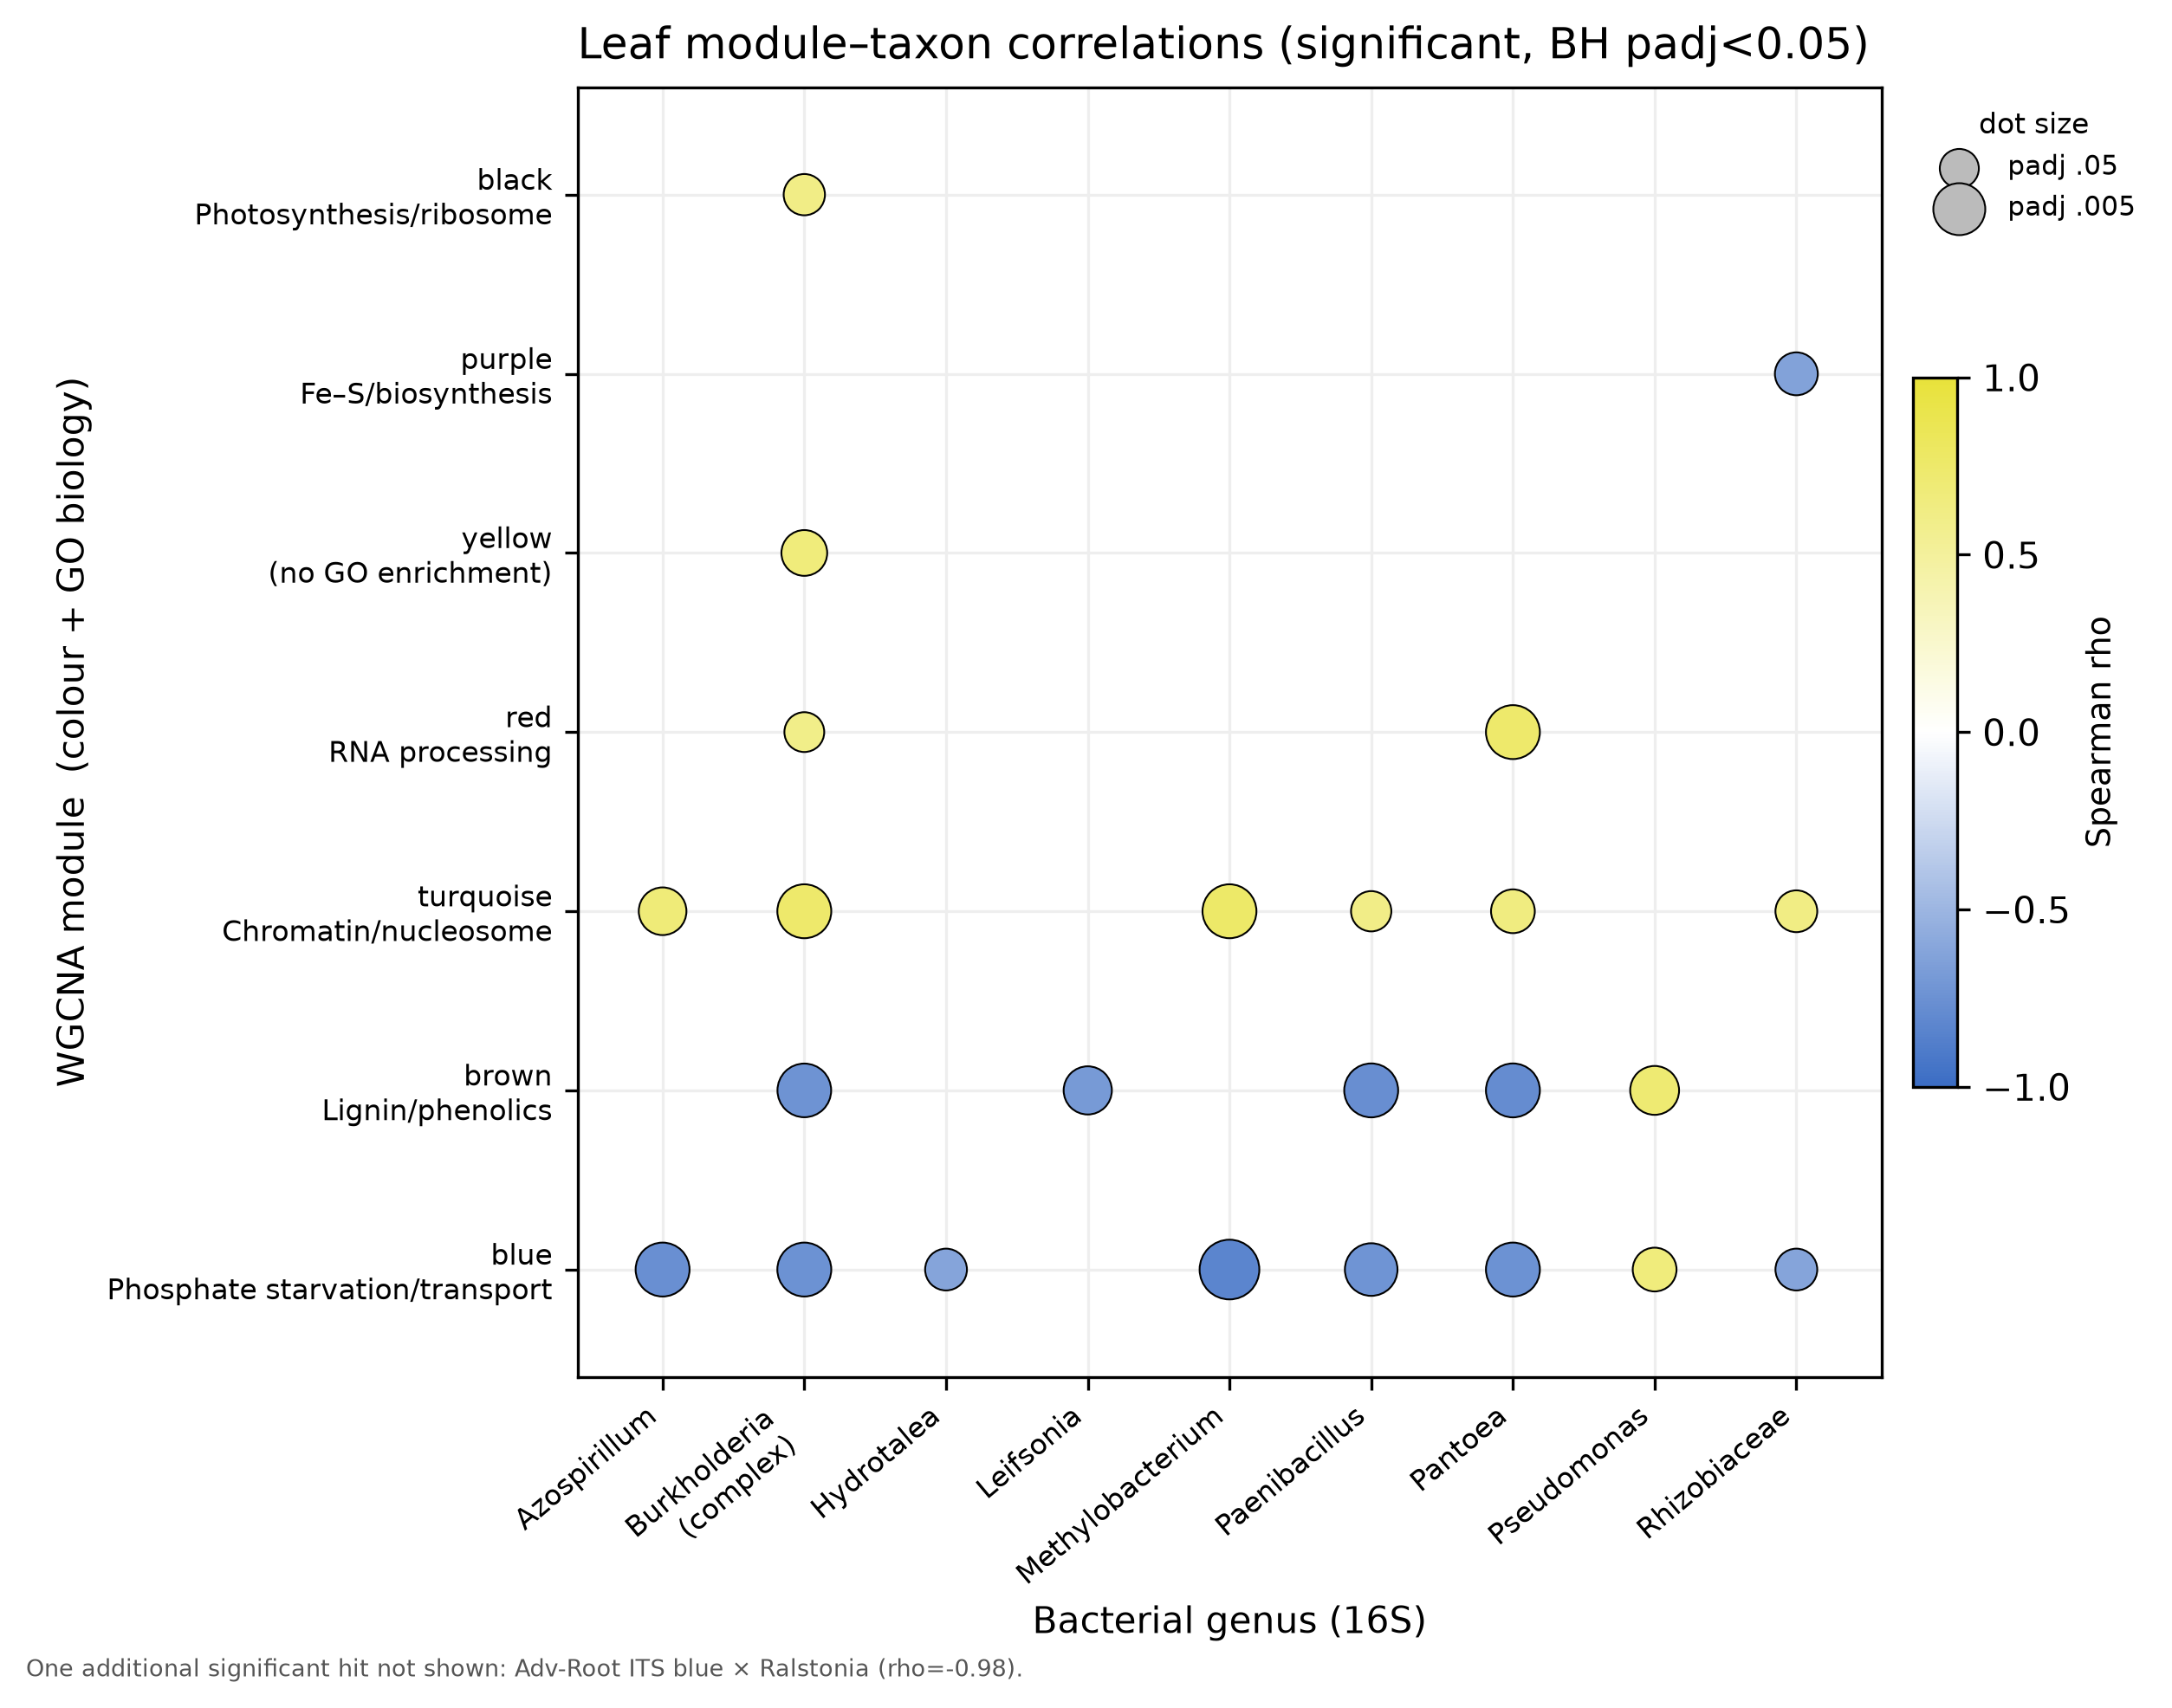
\includegraphics[width=0.85\textwidth]{fig6_module_taxon_network.png}
\caption{\textbf{Leaf module--taxon correlations} (BH \(p_{\mathrm{adj}} < 0.05\)).
The flight-associated turquoise (chromatin/nucleosome) module positively tracks
\textit{Methylobacterium}, \textit{Burkholderia}, and \textit{Azospirillum}, while
the blue (phosphate-starvation) module shows the inverse.}
\label{fig:6}
\end{figure}

\subsection{Functional prediction reveals nitrogen cycling and methanotrophy}
FAPROTAX assigned 239 of 348 bacterial ASVs to 29 functional categories (Table~S6).
The dominant predicted functions were aerobic chemoheterotrophy (787{,}792 reads,
185 taxa), nitrogen fixation (164{,}614 reads, 12 taxa), methanotrophy (96{,}514
reads, 15 taxa), and methanol oxidation (96{,}687 reads, 15 taxa)
(Fig.~\ref{fig:7}). The methanotrophy and methanol oxidation functions were
primarily associated with \textit{Methylobacterium-Methylorubrum}, the same genus
showing the strongest positive correlation with the flight-associated WGCNA module.
Fungal guild assignment (manual genus-level classification) identified saprotrophs
(11 ASVs, dominated by \textit{Penicillium} and \textit{Aspergillus}) and plant
pathogens (2 ASVs: \textit{Fusarium} spp.) as the main guilds (Table~S7).

\begin{figure}[htbp]
\centering
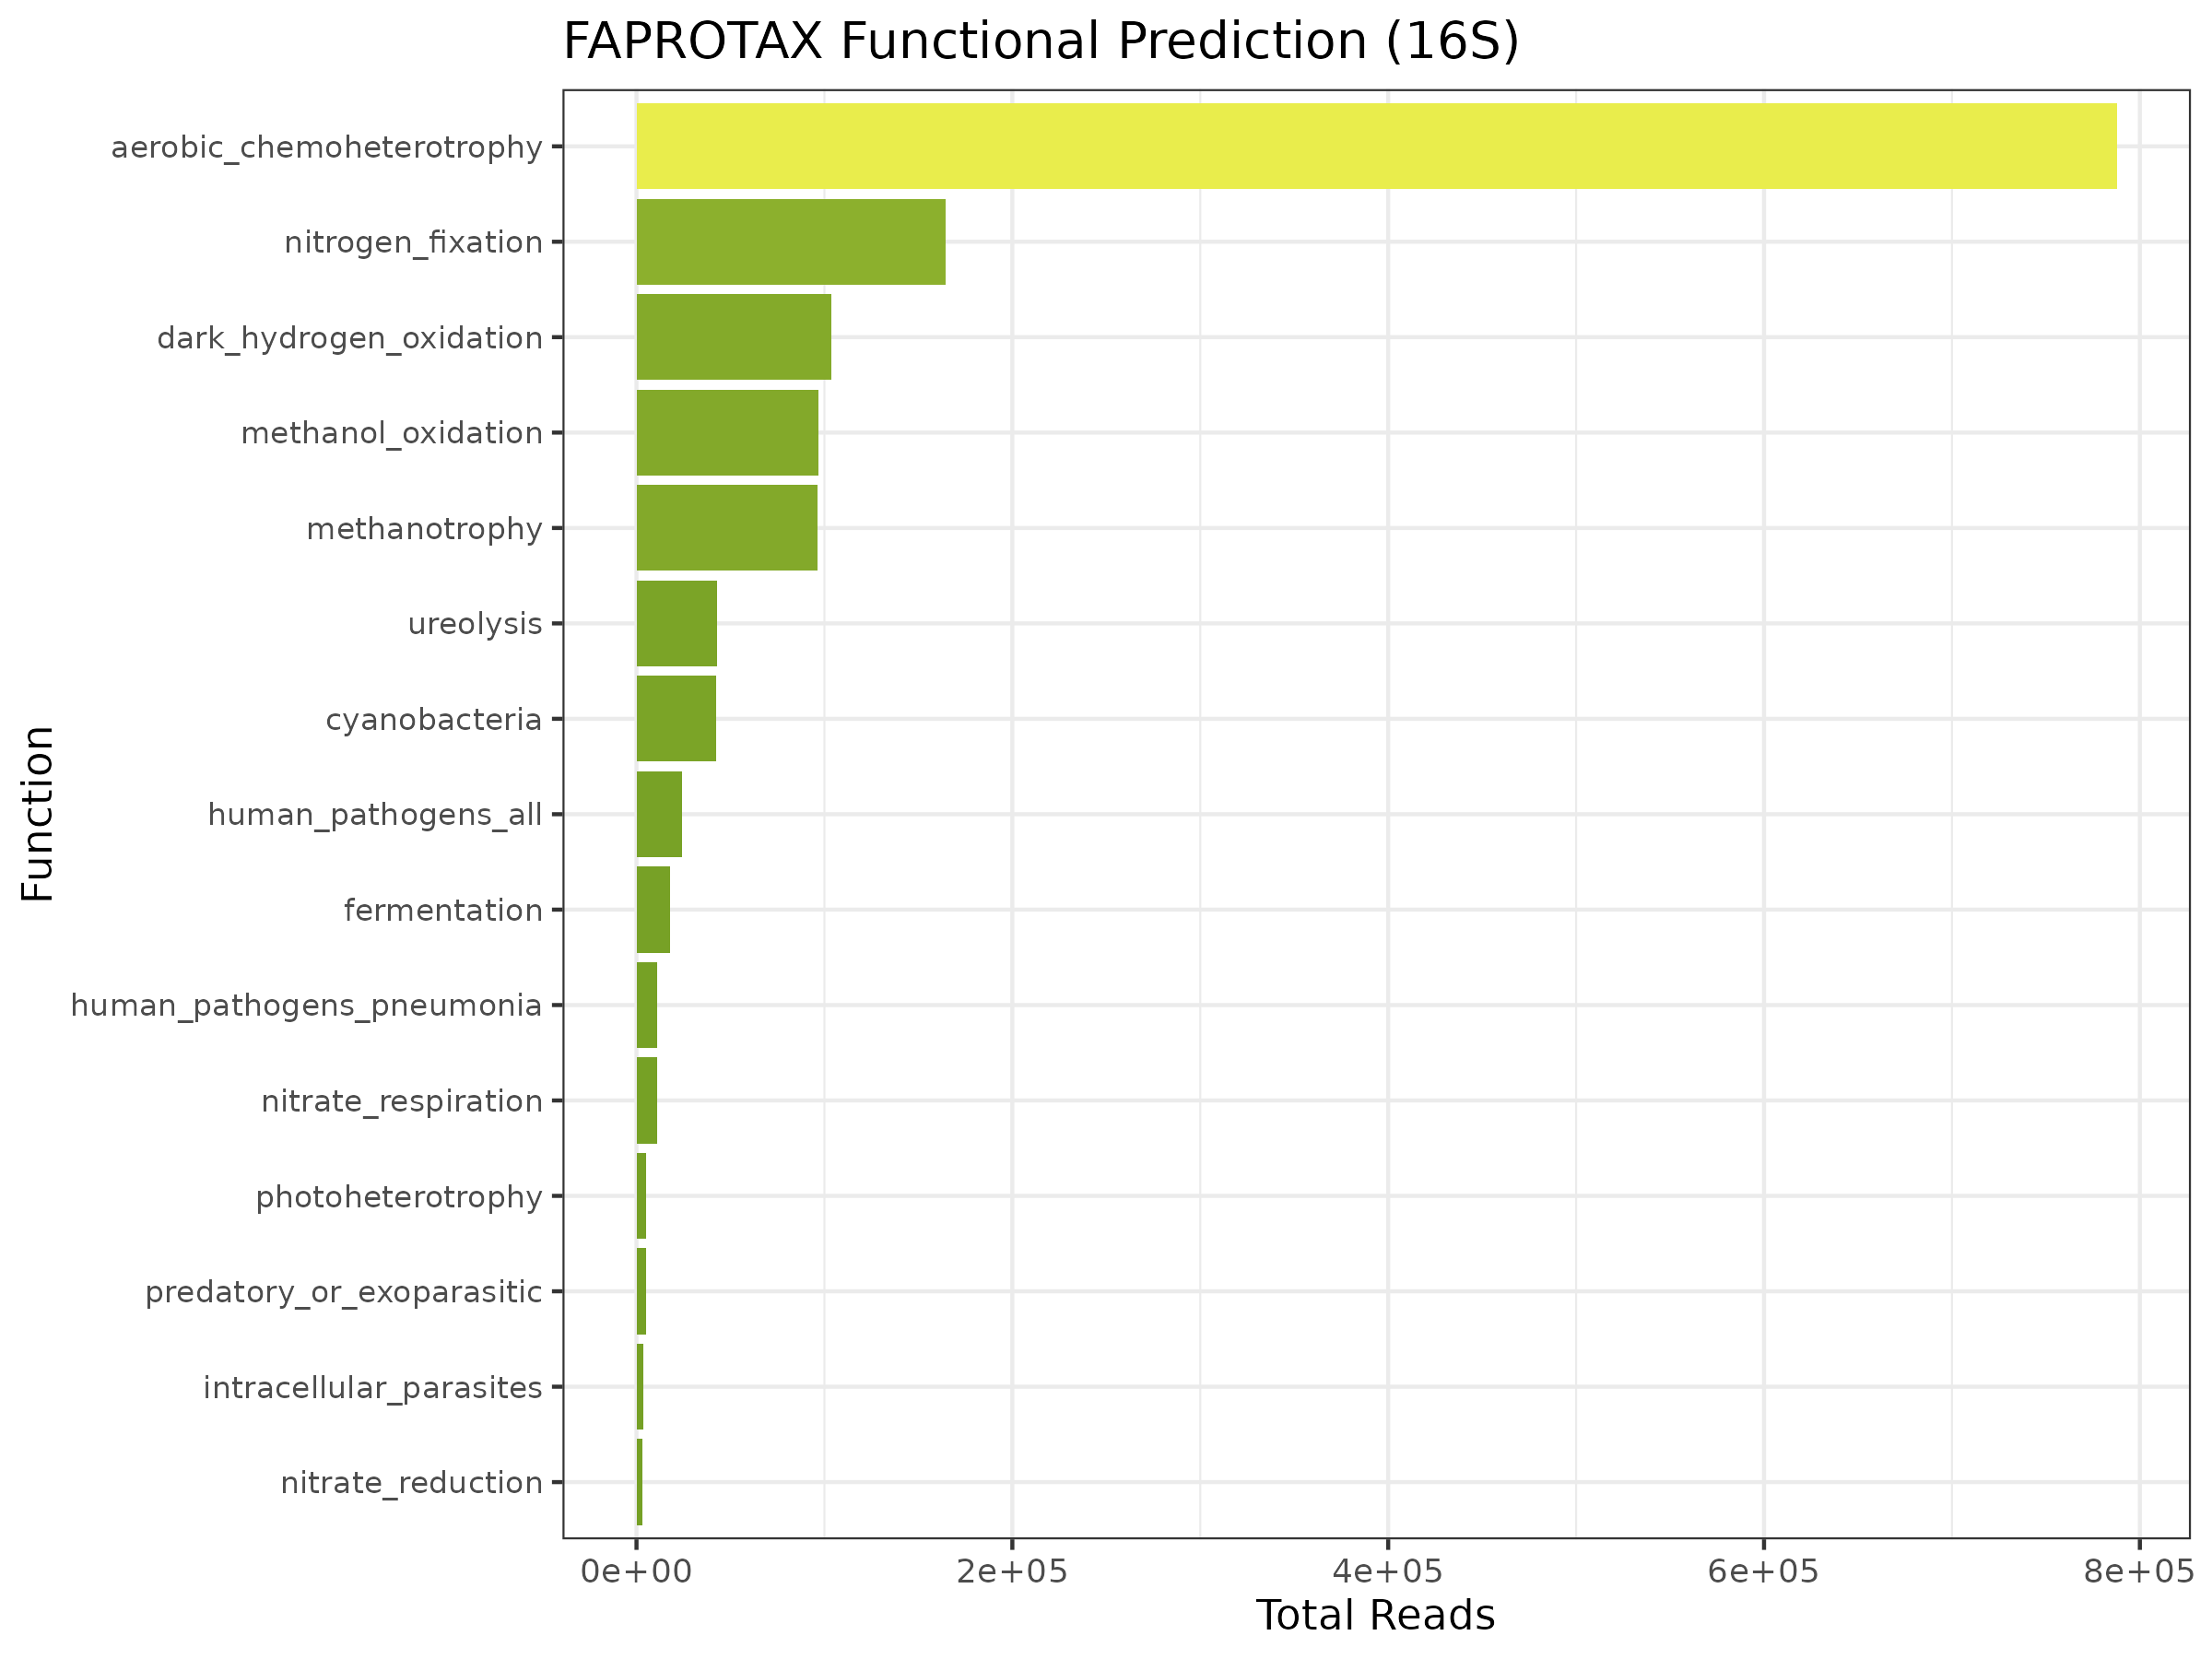
\includegraphics[width=0.8\textwidth]{fig7_faprotax.png}
\caption{\textbf{FAPROTAX predicted bacterial functions} (aerobic chemoheterotrophy,
N fixation, methanotrophy, methanol oxidation).}
\label{fig:7}
\end{figure}

\section{Discussion}\label{sec:discussion}

This study presents the first integrated multi-omics analysis of plant-microbiome
interactions in the ISS VEG-05 experiment. Our findings reveal three key insights:
(1) spaceflight restructures leaf bacterial communities more than fungal
communities, with increased alpha diversity in flight; (2) the host transcriptional
response to spaceflight is strongly light-dependent, particularly in leaves; and (3)
a subset of host genes responds to microbial community changes independently of the
direct spaceflight stimulus, providing evidence for microbe-driven host regulation.

The increased bacterial alpha diversity in flight leaves was initially
counterintuitive, as spaceflight is often associated with reduced microbial
diversity in human microbiome studies \cite{voorhies2019b}. However, in the
phyllosphere, the reduced gravity environment may alter leaf surface properties and
nutrient availability, potentially creating more ecological niches. The strong
correlation between the flight-associated WGCNA module and plant growth-promoting
bacteria (\textit{Methylobacterium}, \textit{Burkholderia}, \textit{Azospirillum})
suggests that spaceflight may favor these beneficial taxa, though the directionality
of this association requires further investigation.

The light-dependent transcriptional response is a novel finding with practical
implications for space crop production. The 9-fold difference in DEG counts between
blue and red light conditions (4{,}716 vs.\ 523) suggests that blue light may
amplify the plant's perception of or response to the spaceflight environment. Blue
light is known to activate cryptochrome photoreceptors and downstream stress
signaling pathways \cite{chaves2011}, which may interact with spaceflight-induced
oxidative stress.

The identification of a microbe-driven WGCNA module in adventitious roots (black
module, 169 genes) is perhaps the most significant finding. This module's strong
correlation with fungal dysbiosis (\(r = -0.85\)) but not with flight status (\(r =
-0.38\), \(p = 0.32\)) indicates that the host transcriptional response in this
module is driven by microbial community changes rather than directly by the
spaceflight environment. Although the black module's own GO enrichment was limited,
the broader adventitious-root oxidative-stress program --- concentrated in the
larger turquoise module --- together with the black module's tight coupling to
fungal dysbiosis suggests that fungal community restructuring may trigger host
defense and redox responses, potentially through oxidative burst signaling.

\subsection{Relationship to a cross-mission salicylic-acid integration}
These microbiome findings dovetail with a companion cross-mission analysis that
integrated the same OSD-767 transcriptome with an Advanced Plant Habitat experiment
manipulating salicylic-acid (SA) signalling (wild-type MoneyMaker versus the
SA-deficient \textit{NahG} line). That analysis concluded that the spaceflight
transcriptome resembles an SA-deficient, biotic-defense-primed state. Our results
offer a proximal explanation: spaceflight-induced dysbiosis --- and the
microbe-driven, flight-independent host module identified here --- could be the
stimulus that elicits that defense-primed signature, with SA acting as the gating
regulator of plant biotic immunity. Both analyses independently recover the
blue-light amplification of the spaceflight response despite using different
pipelines, and this rationalises why gene-level spaceflight signatures replicate
poorly across missions while the biotic-defense \textit{pattern} is conserved. A full
comparison is provided in \texttt{COMPARISON\_with\_SA\_integration.md}.

\subsection{Limitations}
Several limitations should be noted. First, sample sizes are small (\(n = 21\) leaf,
\(n = 15\) root for RNA-seq; \(n = 9\)--12 per group for microbiome), limiting
statistical power. Second, 16S leaf samples had very low bacterial read counts after
host DNA removal (median 89 reads), precluding rarefaction and requiring reliance on
relative abundance metrics. Third, the ITS dataset had uneven group representation,
with some flight groups containing only 1--2 samples. Fourth, MOFA+ warned that
Factor 1 may partially capture technical variation (detection rate differences),
though the strong biological signal supports its interpretation as a flight factor.
Fifth, FAPROTAX functional predictions are taxonomy-based and should be validated
with metagenomic or metatranscriptomic data. Sixth, the FUNGuild analysis used
manual genus-level assignment rather than the full database, reducing assignment
confidence. Finally, this study is correlational; causal relationships between host
transcription and microbiome changes require experimental validation, ideally in
simulated microgravity conditions with microbiome manipulation.

\backmatter

\bmhead{Data and code availability}
All analysis code is available at
\url{https://github.com/dr-richard-barker/veg05-integrated-omics}. Raw data are
available from NASA OSDR (OSD-766, OSD-767).

\bmhead{Acknowledgements}
This work used data from NASA's Open Science Data Repository (OSD-766, OSD-767)
generated by the VEG-05 experiment team. We thank the ISS crew and ground support
teams for sample collection and the GeneLab community for data processing.

\bibliography{references}

\end{document}
